% Options for packages loaded elsewhere
\PassOptionsToPackage{unicode}{hyperref}
\PassOptionsToPackage{hyphens}{url}
%
\documentclass[
  english,
  man, noextraspace]{apa6}
\usepackage{lmodern}
\usepackage{amssymb,amsmath}
\usepackage{ifxetex,ifluatex}
\ifnum 0\ifxetex 1\fi\ifluatex 1\fi=0 % if pdftex
  \usepackage[T1]{fontenc}
  \usepackage[utf8]{inputenc}
  \usepackage{textcomp} % provide euro and other symbols
\else % if luatex or xetex
  \usepackage{unicode-math}
  \defaultfontfeatures{Scale=MatchLowercase}
  \defaultfontfeatures[\rmfamily]{Ligatures=TeX,Scale=1}
\fi
% Use upquote if available, for straight quotes in verbatim environments
\IfFileExists{upquote.sty}{\usepackage{upquote}}{}
\IfFileExists{microtype.sty}{% use microtype if available
  \usepackage[]{microtype}
  \UseMicrotypeSet[protrusion]{basicmath} % disable protrusion for tt fonts
}{}
\makeatletter
\@ifundefined{KOMAClassName}{% if non-KOMA class
  \IfFileExists{parskip.sty}{%
    \usepackage{parskip}
  }{% else
    \setlength{\parindent}{0pt}
    \setlength{\parskip}{6pt plus 2pt minus 1pt}}
}{% if KOMA class
  \KOMAoptions{parskip=half}}
\makeatother
\usepackage{xcolor}
\IfFileExists{xurl.sty}{\usepackage{xurl}}{} % add URL line breaks if available
\IfFileExists{bookmark.sty}{\usepackage{bookmark}}{\usepackage{hyperref}}
\hypersetup{
  pdftitle={The development of infants' responses to mispronunciations: A Meta-Analysis},
  pdfauthor={Katie Von Holzen1,2,3 \& Christina Bergmann4,5},
  pdflang={en-EN},
  pdfkeywords={language acquisition; mispronunciation sensitivity; word recognition; meta-analysis; lexicon; infancy},
  hidelinks,
  pdfcreator={LaTeX via pandoc}}
\urlstyle{same} % disable monospaced font for URLs
\usepackage{graphicx}
\makeatletter
\def\maxwidth{\ifdim\Gin@nat@width>\linewidth\linewidth\else\Gin@nat@width\fi}
\def\maxheight{\ifdim\Gin@nat@height>\textheight\textheight\else\Gin@nat@height\fi}
\makeatother
% Scale images if necessary, so that they will not overflow the page
% margins by default, and it is still possible to overwrite the defaults
% using explicit options in \includegraphics[width, height, ...]{}
\setkeys{Gin}{width=\maxwidth,height=\maxheight,keepaspectratio}
% Set default figure placement to htbp
\makeatletter
\def\fps@figure{htbp}
\makeatother
\setlength{\emergencystretch}{3em} % prevent overfull lines
\providecommand{\tightlist}{%
  \setlength{\itemsep}{0pt}\setlength{\parskip}{0pt}}
\setcounter{secnumdepth}{-\maxdimen} % remove section numbering
% Make \paragraph and \subparagraph free-standing
\ifx\paragraph\undefined\else
  \let\oldparagraph\paragraph
  \renewcommand{\paragraph}[1]{\oldparagraph{#1}\mbox{}}
\fi
\ifx\subparagraph\undefined\else
  \let\oldsubparagraph\subparagraph
  \renewcommand{\subparagraph}[1]{\oldsubparagraph{#1}\mbox{}}
\fi
% Manuscript styling
\usepackage{upgreek}
\captionsetup{font=singlespacing,justification=justified}

% Table formatting
\usepackage{longtable}
\usepackage{lscape}
% \usepackage[counterclockwise]{rotating}   % Landscape page setup for large tables
\usepackage{multirow}		% Table styling
\usepackage{tabularx}		% Control Column width
\usepackage[flushleft]{threeparttable}	% Allows for three part tables with a specified notes section
\usepackage{threeparttablex}            % Lets threeparttable work with longtable

% Create new environments so endfloat can handle them
% \newenvironment{ltable}
%   {\begin{landscape}\begin{center}\begin{threeparttable}}
%   {\end{threeparttable}\end{center}\end{landscape}}
\newenvironment{lltable}{\begin{landscape}\begin{center}\begin{ThreePartTable}}{\end{ThreePartTable}\end{center}\end{landscape}}

% Enables adjusting longtable caption width to table width
% Solution found at http://golatex.de/longtable-mit-caption-so-breit-wie-die-tabelle-t15767.html
\makeatletter
\newcommand\LastLTentrywidth{1em}
\newlength\longtablewidth
\setlength{\longtablewidth}{1in}
\newcommand{\getlongtablewidth}{\begingroup \ifcsname LT@\roman{LT@tables}\endcsname \global\longtablewidth=0pt \renewcommand{\LT@entry}[2]{\global\advance\longtablewidth by ##2\relax\gdef\LastLTentrywidth{##2}}\@nameuse{LT@\roman{LT@tables}} \fi \endgroup}

% \setlength{\parindent}{0.5in}
% \setlength{\parskip}{0pt plus 0pt minus 0pt}

% \usepackage{etoolbox}
\makeatletter
\patchcmd{\HyOrg@maketitle}
  {\section{\normalfont\normalsize\abstractname}}
  {\section*{\normalfont\normalsize\abstractname}}
  {}{\typeout{Failed to patch abstract.}}
\patchcmd{\HyOrg@maketitle}
  {\section{\protect\normalfont{\@title}}}
  {\section*{\protect\normalfont{\@title}}}
  {}{\typeout{Failed to patch title.}}
\makeatother
\shorttitle{Mispronunciation Meta-Analysis}
\keywords{language acquisition; mispronunciation sensitivity; word recognition; meta-analysis; lexicon; infancy}
\DeclareDelayedFloatFlavor{ThreePartTable}{table}
\DeclareDelayedFloatFlavor{lltable}{table}
\DeclareDelayedFloatFlavor*{longtable}{table}
\makeatletter
\renewcommand{\efloat@iwrite}[1]{\immediate\expandafter\protected@write\csname efloat@post#1\endcsname{}}
\makeatother
\usepackage{lineno}

\linenumbers
\usepackage{csquotes}
\usepackage{setspace}
\usepackage{fontspec}
\usepackage{tipa}
\AtBeginEnvironment{tabular}{\singlespacing}
\AtBeginEnvironment{lltable}{\singlespacing}
\AtBeginEnvironment{tablenotes}{\doublespacing}
\captionsetup[table]{font={stretch=1.5}}
\captionsetup[figure]{font={stretch=1.5}}
\captionsetup[table]{font=scriptsize}
\ifxetex
  % Load polyglossia as late as possible: uses bidi with RTL langages (e.g. Hebrew, Arabic)
  \usepackage{polyglossia}
  \setmainlanguage[]{english}
\else
  \usepackage[shorthands=off,main=english]{babel}
\fi
\ifluatex
  \usepackage{selnolig}  % disable illegal ligatures
\fi
\newlength{\cslhangindent}
\setlength{\cslhangindent}{1.5em}
\newenvironment{cslreferences}%
  {\setlength{\parindent}{0pt}%
  \everypar{\setlength{\hangindent}{\cslhangindent}}\ignorespaces}%
  {\par}

\title{The development of infants' responses to mispronunciations: A Meta-Analysis}
\author{Katie Von Holzen\textsuperscript{1,2,3} \& Christina Bergmann\textsuperscript{4,5}}
\date{}


\authornote{

The authors each declare that they have no conflict of interest.

Correspondence concerning this article should be addressed to Katie Von Holzen, Emil-Figge-Straße 50, 44221 Dortmund, Germany. E-mail: \href{mailto:katie.m.vonholzen@gmail.com}{\nolinkurl{katie.m.vonholzen@gmail.com}}

}

\affiliation{\vspace{0.5cm}\textsuperscript{1} Lehrstuhl Linguistik des Deutschen, Schwerpunkt Deutsch als Fremdsprache/Deutsch als Zweitsprache, Technische Universität Dortmund\\\textsuperscript{2} Department of Hearing and Speech Sciences, University of Maryland, USA\\\textsuperscript{3} Laboratoire Psychologie de la Perception, Université Paris Descartes\\\textsuperscript{4} Max Planck Institute for Psycholinguistics, Nijmegen, the Netherlands\\\textsuperscript{5} LSCP, Departement d'Etudes Cognitives, ENS, EHESS, CNRS, PSL Research University}

\abstract{
As they develop into mature speakers of their native language, infants must not only learn words but also the sounds that make up those words. To do so, they must strike a balance between accepting speaker dependent variation (e.g.~mood, voice, accent), but appropriately rejecting variation when it (potentially) changes a word's meaning (e.g.~cat vs.~hat). This meta-analysis focuses on studies investigating infants' ability to detect mispronunciations in familiar words, or mispronunciation sensitivity. Our goal was to evaluate the development of infants' phonological representations for familiar words as well as explore the role of experimental manipulations related to theoretical questions and of analysis choices. The results show that although infants are sensitive to mispronunciations, they still accept these altered forms as labels for target objects. Interestingly, this ability is not modulated by age or vocabulary size, suggesting that a mature understanding of native language phonology may be present in infants from an early age, possibly before the vocabulary explosion. These results support several theoretical assumptions made in the literature, such as sensitivity to mispronunciation size and position of the mispronunciation. We also shed light on the impact of data analysis choices that may lead to different conclusions regarding the development of infants' mispronunciation sensitivity. Our paper concludes with recommendations for improved practice in testing infants' word and sentence processing on-line.
}



\begin{document}
\maketitle

In a mature phono-lexical system, word recognition must balance flexibility to slight variation (e.g., speaker identity, accented speech) while distinguishing between phonological contrasts that differentiate words in a given language (e.g.~cat-hat). This meta-analysis examines the latter, focusing how infants apply the relevant phonological categories of their native language, aggregating twenty years' worth of studies using the mispronunciation sensitivity paradigm. The original study of Swingley and Aslin (2000) presented American-English learning 18- to 23-month-olds with pairs of images of words they were very likely to know (e.g.~a baby and a dog) and their eye movements to each image were recorded. Infants either heard the correct label (e.g.~``baby'') or a mispronounced label (e.g.~``vaby'') for one of the images. Although infants looked at the correct target image in response to both types of labels, correct labels elicited more looking to the target image than mispronounced labels. Swingley and Aslin (2000) concluded that already before the second birthday, children's representations for familiar words are phonologically well specified. As we will review below, there are opposing theories and resulting predictions, supported by empirical data, as to how this knowledge is acquired and applied to lexical representations. The time is thus ripe to aggregate all publicly available evidence using a meta-analysis. In doing so, we can examine developmental trends making use of data from a much larger and diverse sample of infants than is possible in most single studies.

An \emph{increase} in mispronunciation sensitivity with age is predicted by a maturation from holistic to more detailed phono-lexical representations and has been supported by several studies (Altvater-Mackensen, 2010; Altvater-Mackensen, Feest, \& Fikkert, 2014; Feest \& Fikkert, 2015; Mani \& Plunkett, 2007). The first words that infants learn are often not similar sounding (e.g.~mama, ball, kitty; Charles-Luce \& Luce, 1995) and encoding representations for these words using fine phonological detail may not be necessary. According to PRIMIR (Curtin \& Werker, 2007; Werker \& Curtin, 2005) infants' initial episodic representations give way to more abstract phonological word forms, as the infant learns more words, the detail of which can be accessed more or less easily depending on factors such as the infant's age or the demands of the task. This argument is supported by the results of Mani and Plunkett (2010), who found that 12-month-old infants with a larger vocabulary showed a greater sensitivity to vowel mispronunciations than infants with a smaller vocabulary.

Yet, the majority of studies examining a potential association between mispronunciation sensitivity and vocabulary size have concluded that there is no relationship (Bailey \& Plunkett, 2002; Ballem \& Plunkett, 2005; Mani, Coleman, \& Plunkett, 2008; Mani \& Plunkett, 2007; Swingley, 2009; Swingley \& Aslin, 2000, 2002; Zesiger, Lozeron, Levy, \& Frauenfelder, 2012). Furthermore, other studies testing more than one age have found \emph{no difference} in mispronunciation sensitivity (Bailey \& Plunkett, 2002; Swingley \& Aslin, 2000; Zesiger et al., 2012). Such evidence supports an early specificity hypothesis, which suggests continuity in how infants represent familiar words. According to this account, infants represent words with phonological detail already at the onset of lexical acquisition and that this persists throughout development.

There are no theoretical accounts that would predict \emph{decreased} mispronunciation sensitivity, but at least one study has found a decrease in sensitivity to small mispronunciations. Here, 18- but not 24-month-old infants showed sensitivity to more subtle mispronunciations that differed from the correct pronunciation by 1 phonological feature (Mani \& Plunkett, 2011). Mani and Plunkett (2011) argue that when faced with large and salient mispronunciations, infants' sensitivity to small 1-feature mispronunciations may be obscured. This would especially be the case if infants show graded sensitivity to different degrees of mispronunciations (see below), as Mani and Plunkett (2011) found with 24- but not 18-month-olds in their study.

To disentangle the predictions that phono-lexical representations are progressively becoming more specified or are specified early, we investigate the relationship between mispronunciation sensitivity and age as well as vocabulary size by aggregating 20 years of mispronunciation sensitivity studies. But, this may not account for all variability found in the literature. Indeed, different laboratories may vary in their approach to creating a mispronunciation sensitivity experiment, using different types of stimuli and methodologies. Many studies pose more nuanced questions, such as examining the impact of number of phonological features changed (mispronunciation size) or the location of the mispronunciation. Some studies may differ in their experimental design, presenting a distractor image that is either familiar or completely novel. In our meta-analysis we code for features of the experiment that are often reported but vary across studies and include an analysis of these features to shed further light on early phono-lexical representations and their maturation.

These research questions and experimental manipulations have the potential to create experimental tasks that are more or less difficult for the infant to successfully complete. The PRIMIR Framework (Processing Rich Information from Multidimensional Interactive Representations; Curtin \& Werker, 2007; Werker \& Curtin, 2005) describes how infants learn to organize the incoming speech signal into phonetic and indexical detail. The ability to access and use this detail, however, is governed by the task or developmental demands probed in a particular experiment. For example, if infants are tested on a more subtle mispronunciation that changes only one phonological feature, they may be less likely to identify the change in comparison to a mispronunciation that changes two or three phonological features (White \& Morgan, 2008). If older infants are more likely to be tested using a more demanding mispronunciation sensitivity task, this may attenuate developmental effects across studies. Note, however, that those studies we reviewed above reporting change (Altvater-Mackensen, 2010; Altvater-Mackensen et al., 2014; Feest \& Fikkert, 2015; Mani \& Plunkett, 2007) or no change (Bailey \& Plunkett, 2002; Swingley \& Aslin, 2000; Zesiger et al., 2012) all presented the same task across ages.

The first set of questions concerns how infants' sensitivity is modulated by different kinds of mispronunciations. Following on the above example, some experiments examine infants' sensitivity to factors that change the identity of a word on a measurable level, or \emph{mispronunciation size} (i.e.~1-feature, 2-features, 3-features), finding that infants are more sensitive to larger mispronunciations (3-feature-changes) than smaller mispronunciations (1-feature changes) for both consonant (Bernier \& White, 2017; Tamasi, 2016; White \& Morgan, 2008) and vowel (Mani \& Plunkett, 2011) mispronunciations, known as graded sensitivity. By aggregating studies testing infants of different ages on mispronunciations of varying size, this also has consequences for understanding whether graded sensitivity changes over development.

The position of mispronunciation in the word may differentially interrupt the infant's word recognition process, but the degree to which position impacts word recognition is a matter of debate. The COHORT model (Marslen-Wilson \& Zwitserlood, 1989) describes lexical access in a linear direction, with the importance of each phoneme decreasing as its position comes later in the word. In contrast, the TRACE model (McClelland \& Elman, 1986) describes lexical access as constantly updating and reevaluating the incoming speech input in the search for the correct lexical entry, and therefore can recover from word onset and to a lesser extent medial mispronunciations. To evaluate these competing theories, studies often manipulate the \emph{mispronunciation position}, whether onset, medial, or coda, in the word.

Consonantal changes may be more disruptive to lexical processing than vowel changes, known as the consonant bias, and a learned account predicts that this bias emerges over development and is impacted by the language family of the infants' native language (for a review see Nazzi, Poltrock, \& Von Holzen, 2016). Yet, the handful of studies directly comparing sensitivity to consonant and vowel mispronunciations mostly find symmetry as opposed to an asymmetry between consonants and vowels for English- (Mani \& Plunkett, 2007, 2010; but see Swingley, 2016) and Danish-learning infants (Højen et al., n.d.) and do not compare infants learning different native languages (for cross-linguistic evidence from word-learning see Nazzi, Floccia, Moquet, \& Butler, 2009). In the current meta-analysis, we examine infants' sensitivity to the \emph{type of mispronunciation}, whether consonant or vowel, across different ages and native language families to assess the predictions of the learned account of the consonant bias.

A second set of questions is whether the experimental context modulates infants' responses to mispronunciations. In order to study the influence of mispronunciation position, many studies control the \emph{phonological overlap between target and distractor labels}. For example, when examining sensitivity to a vowel mispronunciation of the target word ``ball'', the image of a ball would be paired with a distractor image that shares onset overlap, such as ``bed'', as opposed to a distractor image that does not share onset overlap, such as ``truck''. This ensures that infants cannot use the onset of the word to differentiate between the target and distractor images (Mani \& Plunkett, 2007). Instead, infants must pay attention to the mispronounced phoneme in order to successfully detect the change.

Mispronunciation sensitivity may also be modulated by \emph{distractor familiarity}: whether the distractor used is familiar or unfamiliar. This is a particularly fruitful question to investigate within the context of a meta-analysis, as mispronunciation sensitivity in the presence of a familiar compared to unfamiliar distractor has not been directly compared. Most studies present infants with pictures of two known objects, thereby ruling out the unlabeled competitor, or distractor, as possible target. It is thus not surprising that infants tend to look towards the target more, even when its label is mispronounced. In contrast, other studies present infants with pairs of familiar (labeled target) and unfamiliar (unlabeled distractor) objects (Mani \& Plunkett, 2011; Skoruppa, Mani, Plunkett, Cabrol, \& Peperkamp, 2013; Swingley, 2016; White \& Morgan, 2008). By using an unfamiliar object as a distractor, the infant is presented with a viable option onto which the mispronounced label can be applied (Halberda, 2003; Markman, Wasow, \& Hansen, 2003).

In sum, the studies we have reviewed begin to paint a picture of the development of infants' use of phonological detail in familiar word recognition. Each study contributes one separate brushstroke and it is only by examining all of them together that we can achieve a better understanding of the big picture of early phono-lexical development. Meta-analyses can provide unique insights by estimating the population effect, both of infants' responses to correct and mispronounced labels, and of their mispronunciation sensitivity. Because we aggregate data over age groups, this meta-analysis can investigate the role of maturation by assessing the impact of age, and when possible vocabulary size. We also test the influence of different linguistic (mispronunciation size, position, and type) and contextual (overlap between target and distractor labels; distractor familiarity) factors on the study of mispronunciation sensitivity. Finally, we explore potential data analysis choices that may influence different conclusions about mispronunciation sensitivity development as well as offer recommendations for experiment planning, for example by providing an effect size estimate for a priori power analyses (Bergmann et al., 2018).

\hypertarget{methods}{%
\section{Methods}\label{methods}}

The present meta-analysis was conducted with maximal transparency and reproducibility in mind. To this end, we provide all data and analysis scripts on the supplementary website (\url{https://osf.io/rvbjs/}) and open our meta-analysis up for updates (Tsuji, Bergmann, \& Cristia, 2014). The most recent version is available via the website and the interactive platform MetaLab (\url{https://metalab.stanford.edu}; Bergmann et al., 2018). Since the present paper was written with embedded analysis scripts in R (R Core Team, 2018) using the papaja package (Aust \& Barth, 2018) in R Markdown (Allaire et al., 2018), it is always possible to re-analyze an updated dataset. In addition, we followed the Preferred Reporting Items for Systematic Reviews and Meta-Analyses (PRISMA) guidelines and make the corresponding information available as supplementary materials (Moher, Liberati, Tetzlaff, Altman, \& The\_PRISMA\_Group, 2009). Figure \ref{fig:PRISMA-image} plots our PRISMA flowchart illustrating the paper selection procedure.

(Insert Figure \ref{fig:PRISMA-image} about here)

\begin{figure}
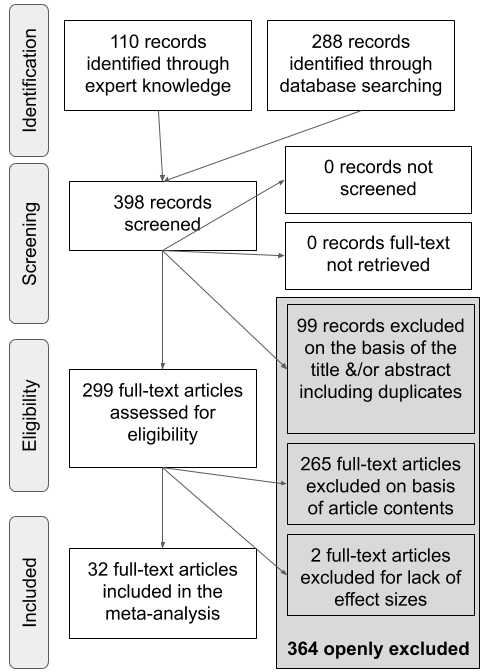
\includegraphics[width=1\linewidth]{figures/Figure_1_PRISMA_MA_Mispronunciation} \caption{A PRISMA flowchart illustrating the selection procedure used to include studies in the current meta-analysis.}\label{fig:PRISMA-image}
\end{figure}

\begin{lltable}

\scriptsize{

\begin{longtable}{llllllllll}\noalign{\getlongtablewidth\global\LTcapwidth=\longtablewidth}
\caption{\label{tab:SummaryTable}Summary of all papers. Age: mean age (in months). Vocabulary: Comp = comprehension, Prod = production. Distractor Familiarity: Fam = Familiar, Unfam = Unfamiliar  Target Overlap: O = onset, M = medial, C = coda. Mispronunciation Size: number of features changed; commas indicate separate comparison, dashes indicate an aggregated range. Mispronunciation Position: O = onset, M = medial, C = coda. Mispronunciation Type: C = consonant, V = vowel, T = tone. A slash separator indicates no distinction was made in the stimuli and unspec. indicates that the value was unspecified in the paper}\\
\toprule
 &  &  &  & \multicolumn{2}{c}{Distractor} & \multicolumn{3}{c}{Mispronunciation}  &\\
\cmidrule(r){5-6} \cmidrule(r){7-9}
Paper & Format & Age & Vocabulary & Familiarity & Target Overlap & Size & Position & Type & N Effect Sizes\\
\midrule
\endfirsthead
\caption*{\normalfont{Table \ref{tab:SummaryTable} continued}}\\
\toprule
 &  &  &  & \multicolumn{2}{c}{Distractor} & \multicolumn{3}{c}{Mispronunciation}  &\\
\cmidrule(r){5-6} \cmidrule(r){7-9}
Paper & Format & Age & Vocabulary & Familiarity & Target Overlap & Size & Position & Type & N Effect Sizes\\
\midrule
\endhead
Altvater-Mackensen (2010) & dissertation & 22, 25 & None & fam, unfam & O, unfam & 1 & O, O/M & C & 13\\
Altvater-Mackensen et al. (2014) & paper & 18, 25 & None & fam & O & 1 & O & C & 16\\
Bailey \& Plunkett (2002) & paper & 18, 24 & Comp & fam & none & 1, 2 & O & C & 12\\
Bergelson \& Swingley (2017) & paper & 7, 9, 12, 6 & None & fam & none & unspec & O/M & V & 9\\
Bernier \& White (2017) & proceedings & 21 & None & unfam & unfam & 1, 2, 3 & O & C & 4\\
Delle Luche et al. (2015) & paper & 20, 19 & None & fam & O & 1 & O & C/V & 4\\
Durrant et al. (2014) & paper & 19, 20 & None & fam & O & 1 & O & C/V & 4\\
Højen et al. (n.d.) & gray paper & 19, 20 & Comp/Prod & fam & C, O & 2-3 & O/M, C/M & C/V, V, C & 6\\
Höhle et al. (2006) & paper & 18 & None & fam & none & 1 & O & C & 4\\
Mani \& Plunkett (2007) & paper & 15, 18, 24, 14, 20 & Comp/Prod & fam & O & 1-2, 1 & O & V, C/V, C & 14\\
Mani \& Plunkett (2010) & paper & 12 & Comp & fam & O & 1 & M, O & V, C & 8\\
Mani \& Plunkett (2011) & paper & 23, 17 & None & unfam & unfam & 1-3, 1, 2, 3 & M & V & 15\\
Mani, Coleman, \& Plunkett (2008) & paper & 18 & Comp/Prod & fam & O & 1 & M & V & 4\\
Ramon-Casas \& Bosch (2010) & paper & 24, 25 & None & fam & none & unspec & M & V & 4\\
Ramon-Casas et al. (2009) & paper & 21, 20 & Prod & fam & none & unspec & M & V & 10\\
Ren \& Morgan (in press) & gray paper & 19 & None & unfam & none & 1 & O, C & C & 8\\
Skoruppa et al. (2013) & paper & 23 & None & unfam & O/M & 1 & C & C & 4\\
Swingley \& Aslin (2000) & paper & 20 & Comp & fam & none & 1 & O & C/V & 2\\
Swingley \& Aslin (2002) & paper & 15 & Comp/Prod & fam & none & 1, 2 & O/M & C/V & 4\\
Swingley (2003) & paper & 19 & Comp/Prod & fam & O & 1 & O, M & C & 6\\
Swingley (2009) & paper & 17 & Comp/Prod & fam & none & 1 & O, C & C & 4\\
Swingley (2016) & paper & 27, 28 & Prod & unfam & unfam & 1 & O/M & C/V, C, V & 9\\
Tamasi (2016) & dissertation & 30 & None & unfam & unfam & 1, 2, 3 & O & C & 4\\
Tao \& Qinmei (2013) & paper & 12 & None & fam & none & unspec & unspec & T & 4\\
Tao et al. (2012) & paper & 16 & Comp & fam & none & unspec & unspec & T & 6\\
van der Feest \& Fikkert, (2015) & paper & 24, 20 & None & fam & O & 1 & O & C & 16\\
van der Feest \& Johnson (2016) & paper & 24 & None & fam & O & 1 & O & C & 20\\
Wewalaarachchi et al. (2017) & paper & 24 & None & unfam & unfam & 1 & O/M/C & C/V/T, V, C, T & 8\\
White \& Aslin (2011) & paper & 18 & None & unfam & unfam & 1 & M & V & 4\\
White \& Morgan (2008) & paper & 18, 19 & None & unfam & unfam & 1, 2, 3 & O & C & 12\\
Zesiger \& Jöhr (2011) & paper & 14 & None & fam & none & 1 & O, M & C, V & 7\\
Zesiger et al. (2012) & paper & 12, 19 & Comp/Prod & fam & none & 1, 2 & O & C & 6\\
\bottomrule
\end{longtable}

}

\end{lltable}

\hypertarget{study-selection}{%
\subsection{Study Selection}\label{study-selection}}

We first generated a list of potentially relevant items to be included in our meta-analysis by creating an expert list (see Figure \ref{fig:PRISMA-image} for an overview of the selection process). This process yielded 110 items. We then used the Google Scholar search engine to search for papers citing the original Swingley and Aslin (2000) publication. This search was conducted on 22 September, 2017 and yielded 288 results. From this combined list of 398 records we removed 99 duplicate items and screened the remaining 299 items for their title and abstract to determine whether each met the following inclusion criteria: (1) original data was reported; (2) the experiment examined familiar word recognition and mispronunciations; (3) infants studied were under 31-months-of-age and typically developing; (4) the dependent variable was derived from proportion of looks to a target image versus a distractor in a eye movement experiment; (5) the stimuli were auditory speech. The final sample (\emph{n} = 32) consisted of 27 journal articles, 1 proceedings paper, 2 theses, and 2 unpublished reports. We will refer to these items collectively as papers. Table \ref{tab:SummaryTable} provides an overview of all papers included in the present meta-analysis.

(Insert Table 1 about here)

\hypertarget{data-entry}{%
\subsection{Data Entry}\label{data-entry}}

The 32 papers we identified as relevant were then coded with as much consistently reported detail as possible (Bergmann et al., 2018; Tsuji et al., 2014). For each experiment (note that a paper typically has multiple experiments), we entered variables describing the publication, population, experiment design and stimuli, and results. For the planned analyses to evaluate the development of mispronunciation sensitivity and modulating factors, we focus on the following characteristics: 1) Condition: Were words mispronounced or not; 2) Mean age reported per group of infants, in days; 3) Vocabulary size, measured by a standardized questionnaire or list; 4) Size of mispronunciation, measured in features changed; 5) Position of mispronunciation: onset, medial, coda; 6) Type of mispronunciation: consonant, vowel, or both; 7) Phonological overlap between target and distractor: onset, medial, coda, none; 8) Distractor familiarity: familiar or unfamiliar. A detailed explanation for moderating factors 3-8 can be found in their respective sections in the Results.\footnote{Two papers tested bilingual infants (Ramon-Casas \& Bosch, 2010; Ramon-Casas, Swingley, Sebastián-Gallés, \& Bosch, 2009), yielding 2 and 4 records, respectively. Due to this small number, we do not investigate the role of multilingualism, but do note that removing these papers from the meta-analysis did not alter the pattern of results.} We separated conditions according to whether or not the target word was mispronounced to be able to investigate infants' looking to the target picture as well as their mispronunciation sensitivity, which is the difference between looks to the target in correct and mispronounced trials. When the same infants were further exposed to multiple mispronunciation conditions and the results were reported separately in the paper, we also entered each condition as a separate row (e.g., consonant versus vowel mispronunciations; Mani \& Plunkett, 2007). The fact that the same infants contributed data to multiple rows (minimally those containing information on correct and mispronounced trials) leads to shared variance across effect sizes, which we account for in our analyses (see next section). We will call each row a record; in total there were 251 records in our data.

\hypertarget{data-analysis}{%
\subsection{Data analysis}\label{data-analysis}}

Effect sizes are reported for infants' looks to target pictures after hearing a correctly pronounced or a mispronounced label (object identification) as well as the difference between effect sizes for correct and mispronounced trials (i.e.~mispronunciation sensitivity). The effect size reported in the present paper is based on comparison of means, standardized by their variance. The most well-known effect size from this group is Cohen's \emph{d} (Cohen, 1988). To correct for the small sample sizes common in infant research, however, we used Hedges' \emph{g} instead of Cohen's \emph{d} (Hedges, 1981; Morris \& DeShon, 2002).

We calculated Hedges' \emph{g} using the raw means and standard deviations reported in the paper (\emph{n} = 177 records from 25 papers) or reported t-values (\emph{n} = 74 records from 9 papers). Two papers reported raw means and standard deviations for some records and just t-values for the remaining records (Altvater-Mackensen et al., 2014; Swingley, 2016). Raw means and standard deviations were extracted from figures for 3 papers. In a within-participant design, when two means are compared (i.e.~looking during pre- and post-naming) it is necessary to obtain correlations between the two measurements at the participant level to calculate effect sizes and effect size variance. Upon request we were provided with correlation values for one paper (Altvater-Mackensen, 2010); we were able to compute correlations using means, standard deviations, and t-values for 5 papers (following Csibra, Hernik, Mascaro, Tatone, \& Lengyel, 2016; see also Rabagliati, Ferguson, \& Lew-Williams, 2018). Correlations were imputed for the remaining papers (Bergmann \& Cristia, 2016). For two papers, we could not derive any effect size (Ballem \& Plunkett, 2005; Renner, 2017), and for a third paper, we do not have sufficient information in one record to compute effect sizes (Skoruppa et al., 2013). We compute a total of 106 effect sizes for correct pronunciations and 150 for mispronunciations. Following standard meta-analytic practice, we remove outliers, i.e.~effect sizes more than 3 standard deviations from the respective mean effect size. This leads to the exclusion of 2 records for correct pronunciations and 3 records for mispronunciations.

To consider the fact that the same infants contributed to multiple datapoints, we analyze our results in a multilevel approach using the R (R Core Team, 2018) package metafor (Viechtbauer, 2010). We use a multilevel random effects model which estimates the mean and variance of effect sizes sampled from an assumed distribution of effect sizes. In the random effect structure we take into account the shared variance of effect sizes drawn from the same paper, and nested therein that the same infants might contribute to multiple effect sizes.

Mispronunciation sensitivity studies typically examine infants' proportion of target looks (PTL) in comparison to some baseline measurement. PTL is calculated by dividing the percentage of looks to the target by the total percentage of looks to both the target and distractor images. Across papers the baseline comparison varied; since other options were not available to us, we used the baseline reported by the authors of each paper. Over half of the records (\emph{n} = 129) subtracted the PTL score for a pre-naming phase from the PTL score for a post-naming phase, resulting in a Difference Score. The Difference Score is one value, which is then compared with a chance value of 0. Pre vs.~Post (\emph{n} = 69 records) accomplishes the same analysis, directly compare the post- and pre-naming PTL scores with one another using a statistical test (e.g.~t-test, ANOVA). This requires two values, one for the pre-naming phase and one for the post-naming phase. The remaining records used a Post dependent variable (\emph{n} = 53 records), which compares the post-naming PTL score with a chance value of 50\%. Here, the infants' pre-naming phase baseline preferences are not considered and instead target fixations are evaluated based on the likelihood to fixate one of two pictures (50\%). Standardized effect sizes based on mean differences, as calculated here, preserve the sign. Consequently, positive effect sizes reflect more looks to the target picture after naming, and larger positive effect sizes indicate comparatively more looks to the target.

Finally, we assess the statistical power of studies included in our meta-analysis, as well as calculate the sample size required to achieve a 80\% power considering our estimate of the population effect and its variance. Failing to take effect sizes into account can lead to either underpowered research or testing too many participants. Underpowered studies will lead to false negatives more frequently than expected, which in turn results in an unpublished body of literature (Bergmann et al., 2018). At the same time, underpowered studies with significant outcomes are likely to overestimate the effect, leading to wrong estimations of the population effect when paired with publication bias (Jennions, Mù, Pierre, Curie, \& Cedex, 2002). Overpowered studies mean that participants were tested unnecessarily, which has ethical implications particularly when working with infants and other difficult to recruit and test populations.

\hypertarget{publication-bias}{%
\subsection{Publication Bias}\label{publication-bias}}

In the psychological sciences, there is a documented reluctance to publish null results. As a result, significant results tend to be over-reported and thus might be over-represented in our meta-analyses (see Ferguson \& Heene, 2012). To examine whether this is also the case in the mispronunciation sensitivity literature, which would bias the data analyzed in this meta-analysis, we conducted two tests. We first examined whether effect sizes are distributed as expected based on sampling error using the rank correlation test of funnel plot asymmetry with the R (R Core Team, 2018) package metafor (Viechtbauer, 2010). Effect sizes with low variance were expected to fall closer to the estimated mean, while effect sizes with high variance should show an increased, evenly-distributed spread around the estimated mean. Publication bias would lead to an uneven spread.

Second, we analyze all of the significant results in the dataset using a p-curve from the p-curve app (v4.0, \url{http://p-curve.com}; Simonsohn, Nelson, \& Simmons, 2014). This p-curve tests for evidential value by examining whether the p-values follow the expected distribution of a right skew in case the alternative hypothesis is true, versus a flat distribution that speaks for no effect being present in the population and all observed significant effects being spurious.

Responses to correctly pronounced and mispronounced labels were predicted to show different patterns of looking behavior. In other words, there is an expectation that infants should look to the target when hearing a correct pronunciation, but studies vary in their report of significant looks to the target when hearing a mispronounced label (i.e.~there might be no effect present in the population); as a result, we conducted these two analyses to assess publication bias separately for both conditions.

\hypertarget{meta-analysis}{%
\subsection{Meta-analysis}\label{meta-analysis}}

The models reported here are multilevel random-effects models of variance-weighted effect sizes, which we computed with the R (R Core Team, 2018) package metafor (Viechtbauer, 2010). To investigate how development impacts mispronunciation sensitivity, our core theoretical question, we first introduced age (centered; continuous and measured in days but transformed into months for ease of interpreting estimates by dividing by 30.44) as a moderator to our main model. Second, we analyzed the correlation between reported vocabulary size and mispronunciation sensitivity using the package meta (Schwarzer, 2007). For a subsequent investigation of experimental characteristics, we introduced each separately as a moderator: size of mispronunciation, position of mispronunciation, type of mispronunciation, phonological overlap between target and distractor labels, and distractor familiarity (more detail below).

\hypertarget{results}{%
\section{Results}\label{results}}

\hypertarget{publication-bias-1}{%
\subsection{Publication Bias}\label{publication-bias-1}}

Figure \ref{fig:FunnelCombo} shows the funnel plots for both correct pronunciations and mispronunciations (code adapted from Sakaluk, 2016). Funnel plot asymmetry was significant for both correct pronunciations (Kendall's \(\tau\) = 0.52, \emph{p} \textless{} .001) and mispronunciations (Kendall's \(\tau\) = 0.16, \emph{p} = 0.005). These results, quantifying the asymmetry in the funnel plots (Figure \ref{fig:FunnelCombo}), indicate bias in the literature. This is particularly evident for correct pronunciations, where larger effect sizes have greater variance (bottom right corner) and the more precise effect sizes (i.e.~smaller variance) tend to be smaller than expected (top left, outside the triangle).

The stronger publication bias for correct pronunciation might reflect the status of this condition as a control. If infants were not looking to the target picture after hearing the correct label, the overall experiment design is called into question. However, even in a well-powered study one would expect the regular occurrence of null results even though as a population, infants would reliably show the expected object identification effect.

We should also point out that funnel plot asymmetry can be caused by multiple factors besides publication bias, such as heterogeneity in the data. There are various possible sources of heterogeneity, which our subsequent moderator analyses will begin to address. Nonetheless, we will remain cautious in our interpretation of our findings and hope that an open dataset which can be expanded by the community will attract previously unpublished null results so we can better understand infants' developing mispronunciation sensitivity.

\begin{figure}
\centering
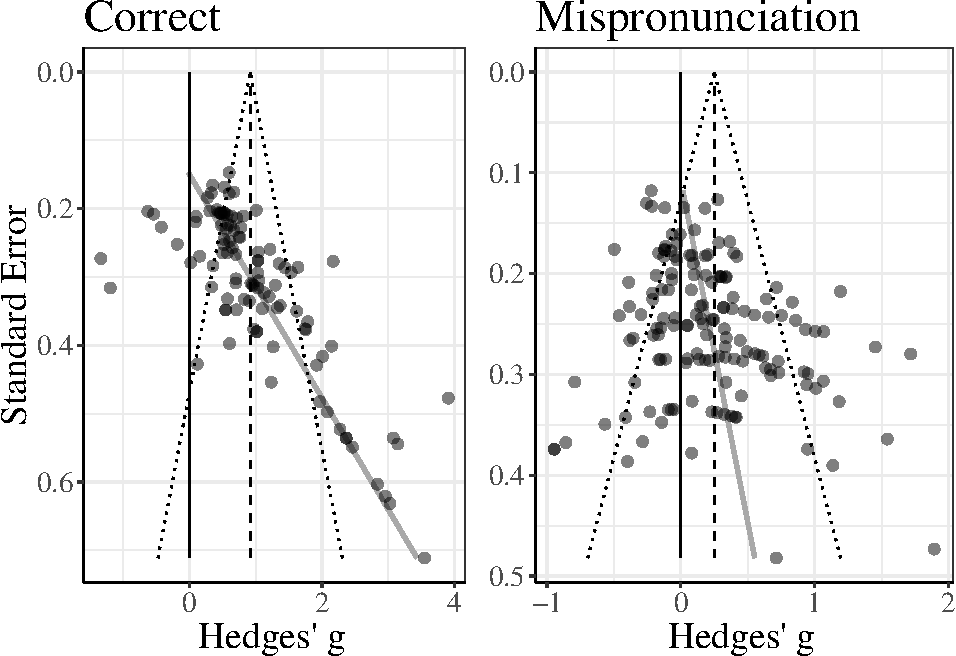
\includegraphics{VonHolzenBergmann_MPMetaAnalysis_files/figure-latex/FunnelCombo-1.pdf}
\caption{\label{fig:FunnelCombo}Funnel plots for object identification, plotting the standard error of the effect size in relation to the effect size. The black line marks zero, the dashed grey line marks the effect estimate, and the grey line marks funnel plot asymmetry.}
\end{figure}

(Insert Figure \ref{fig:FunnelCombo} about here)

We next examined the p-curves for significant values from the correctly pronounced and mispronounced conditions. The p-curve based on 72 statistically significant values for correct pronunciations indicates that the data contain evidential value (Z = -17.93, \emph{p} \textless{} .001) and we find no evidence of a large proportion of p-values just below the typical alpha threshold of .05 that researchers consistently apply in this line of research. The p-curve based on 36 statistically significant values for mispronunciations indicates that the data contain evidential value (Z = -6.81, \emph{p} \textless{} .001) and there is again no evidence of a large proportion of p-values just below the typical alpha threshold of .05.

Taken together, the results suggest a tendency in the literature towards publication bias. As a result, our meta-analysis may systematically overestimate effect sizes and we therefore interpret all estimates with caution. Yet, the p-curve analysis suggests that the literature contains evidential value, reflecting a ``real'' effect. We therefore continue our meta-analysis.

\hypertarget{meta-analysis-1}{%
\subsection{Meta-analysis}\label{meta-analysis-1}}

\hypertarget{object-identification-for-correct-and-mispronounced-words}{%
\subsubsection{Object Identification for Correct and Mispronounced Words}\label{object-identification-for-correct-and-mispronounced-words}}

We first calculated the meta-analytic effect for infants' ability to identify objects when hearing correctly pronounced labels. The variance-weighted meta-analytic effect size Hedges' \emph{g} was 0.919 (SE = 0.122), a large effect, which was significantly different from zero (CI {[}0.679, 1.158{]}, \emph{p} \textless{} .001) with a CI lower bound of 0.68. We then calculated the meta-analytic effect for object identification in response to mispronounced words. In this case, the variance-weighted meta-analytic effect size was 0.251 (SE = 0.06), a small effect, which was also significantly different from zero (CI {[}0.134, 0.368{]}, \emph{p} \textless{} .001). When presented with a correct or mispronounced label, infants fixated the correct object.

\hypertarget{mispronunciation-sensitivity-meta-analytic-effect}{%
\subsubsection{Mispronunciation Sensitivity Meta-Analytic Effect}\label{mispronunciation-sensitivity-meta-analytic-effect}}

The above two analyses considered the data from mispronounced and correctly pronounced words separately. To evaluate mispronunciation sensitivity, we compared the effect size Hedges' \emph{g} for correct pronunciations with mispronunciations directly. To this end, we combined the two datasets. When condition was included (correct, mispronounced), the moderator test was significant (QM(1) = 102.114, \emph{p} \textless{} .001). The estimate for mispronunciation sensitivity was 0.606 (SE = 0.06), and infants' looking behavior across conditions was significantly different (CI {[}0.489, 0.724{]}, \emph{p} \textless{} .001). This confirms that although infants fixate the correct object for both correct pronunciations and mispronunciations, the observed fixations to target (as measured by the effect sizes) were significantly greater for correct pronunciations, suggesting sensitivity to mispronunciations.

The estimated effect for mispronunciation sensitivity in this meta-analysis is 0.61, and the median sample size is 24 participants. If we were to assume that researchers assess mispronunciation sensitivity in a simple paired t-test, the resulting power is 54\%. In other words, only about half the studies should report a significant result even with a true population effect. Reversely, to achieve 80\% power, one would need to test 44 participants.

Heterogeneity was significant for both correctly pronounced (Q(103) = 626.38, \emph{p} \textless{} .001) and mispronounced words, (Q(146) = 466.45, \emph{p} \textless{} .001), as well as mispronunciation sensitivity, which included the moderator condition (QE(249) = 1,092.83, \emph{p} \textless{} .001). This indicated that the sample contains unexplained variance leading to significant difference between studies beyond what is to be expected based on random sampling error. In our moderator analysis we investigate possible sources of this variance.

\hypertarget{object-recognition-and-mispronunciation-sensitivity-modulated-by-age}{%
\subsubsection{Object Recognition and Mispronunciation Sensitivity Modulated by Age}\label{object-recognition-and-mispronunciation-sensitivity-modulated-by-age}}

To evaluate the different predictions we laid out in the introduction for how mispronunciation sensitivity will change as infants develop, we next added the moderator age (centered; continuous and measured in days but transformed into months for ease of interpreting estimates by dividing by 30.44 for Figure \ref{fig:PlotMPEffect}).

In the first analyses, we investigate the impact of age separately on conditions where words were either pronounced correctly or not. Age did not significantly modulate object identification in response to correctly pronounced (QM(1) = 0.537, \emph{p} = 0.464) or mispronounced words (QM(1) = 1.663, \emph{p} = 0.197). The lack of a significant modulation together with the small estimates for age (correct: \(\beta\) = 0.014, SE = 0.019, 95\% CI{[}-0.023, 0.05{]}, \emph{p} = 0.464; mispronunciation: \(\beta\) = 0.015, SE = 0.011, 95\% CI{[}-0.008, 0.037{]}, \emph{p} = 0.197) indicates that there was no relationship between age and target looks in response to a correctly pronounced or mispronounced label. However, previous experimental studies (e.g.~Fernald, Pinto, Swingley, Weinberg, \& McRoberts, 1998) and a recent meta-analysis (Frank, Lewis, \& Macdonald, 2016) have found that children's speed and accuracy in recognition of correctly pronounced words increases with age. Perhaps older children are more likely to be tested on less-frequent, later learned words than younger children, which could lead to a lack of a relationship between age and target looks in response to correct pronunciations in the current meta-analysis.

We then examined the interaction between age and mispronunciation sensitivity (correct vs.~mispronounced words) in our whole dataset. The moderator test was significant (QM(3) = 104.837, \emph{p} \textless{} .001). The interaction between age and mispronunciation sensitivity, however, was not significant (\(\beta\) = 0.012, SE = 0.013, 95\% CI{[}-0.014, 0.038{]}, \emph{p} = 0.361). The small estimate, as well as inspection of Figure \ref{fig:PlotMPEffect}, suggests that as infants age, their mispronunciation sensitivity neither increases or decreases.

(Insert Figure \ref{fig:PlotMPEffect} about here)

\begin{figure}
\centering
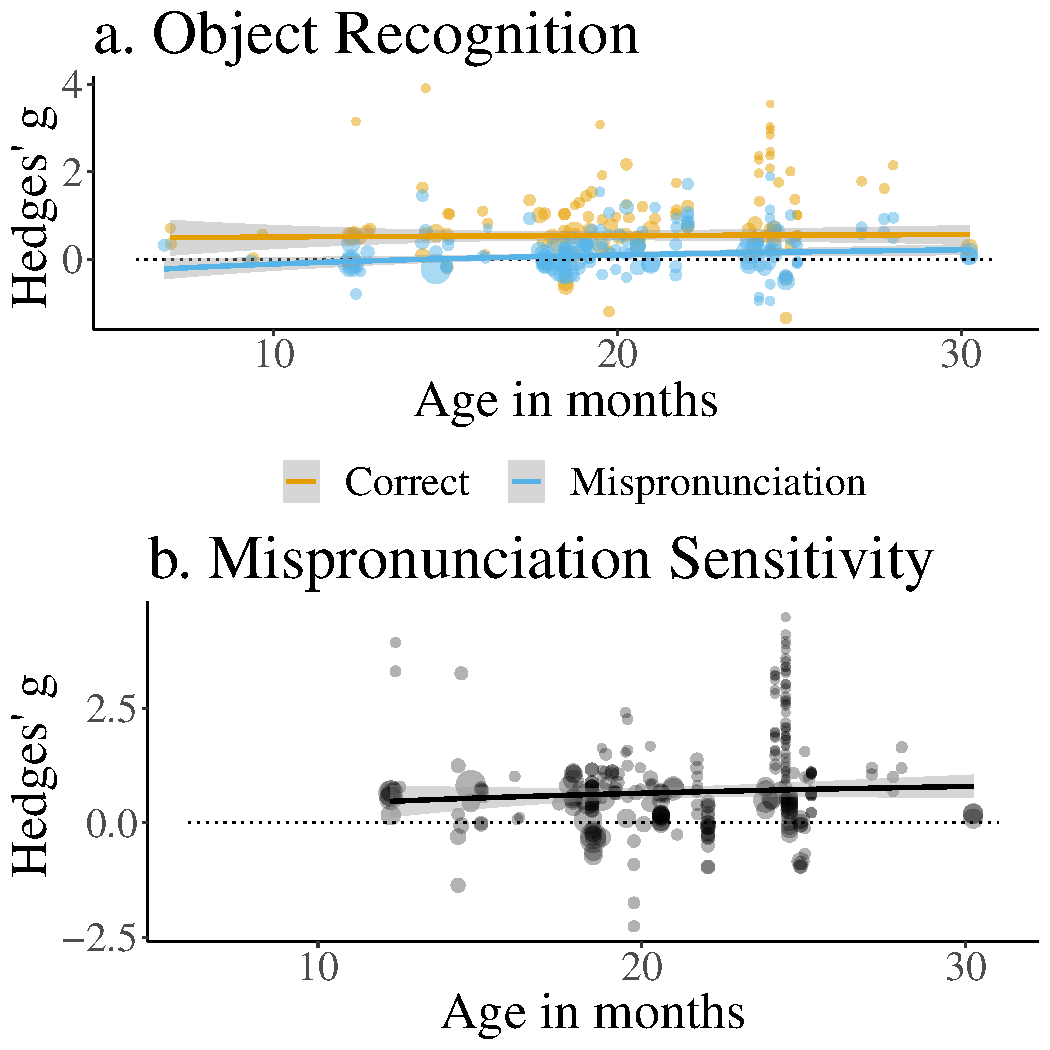
\includegraphics{VonHolzenBergmann_MPMetaAnalysis_files/figure-latex/PlotMPEffect-1.pdf}
\caption{\label{fig:PlotMPEffect}Panel a: Effect sizes for correct pronunciations (yellow) and mispronunciations (blue) by participant age. Panel b: Effect sizes for mispronunciation sensitivity within subject group and study (correct - mispronunciations) by participant age. For both panels, point size depicts inverse variance and the dashed line indicates zero (chance).}
\end{figure}

\hypertarget{vocabulary-correlations}{%
\subsubsection{Vocabulary Correlations}\label{vocabulary-correlations}}

Children comprehend more words than they can produce, leading to different estimates for comprehension and production and we planned to analyze these correlations separately. Of the 32 papers included in the meta-analysis, 13 analyzed the relationship between vocabulary scores and object recognition for correct pronunciations and mispronunciations (comprehension = 11 papers and 39 records; production = 3 papers and 20 records). Although production data may be easier to estimate for parents in the typical questionnaire-based assessment, we deemed 3 papers for production correlations too few to analyze. We also note that individual effect sizes in our analysis were related to object recognition and not mispronunciation sensitivity, and we therefore focus exclusively on the relationship between comprehension and object recognition for correct pronunciations and mispronunciations.

We first considered the relationship between vocabulary and object recognition for correct pronunciations. Higher comprehension scores were associated with greater object recognition in response to correct pronunciations for 9 of 10 records, with correlation values ranging from -0.16 to 0.48. The weighted mean effect size Pearson's \emph{r} of 0.14 was small but did differ significantly from zero (CI {[}0.03; 0.25{]} \emph{p} = 0.012). As a result, we can draw a tentative conclusion that there is a positive relationship between comprehension scores and object recognition in response to correct pronunciations.

We next considered the relationship between vocabulary and object recognition for mispronunciations. Higher comprehension scores were associated with greater object recognition in response to mispronunciations for 17 of 29 records, with correlation values ranging from -0.35 to 0.57. The weighted mean effect size Pearson's \emph{r} of 0.05 was small and did not differ significantly from zero (CI {[}-0.01; 0.12{]} \emph{p} = 0.119). The small correlation suggests either a very small positive or no relationship between vocabulary and object recognition for mispronunciations.

Figure \ref{fig:Vocabdescribe1} plots the year of publication for all the mispronunciation sensitivity studies included in this meta-analysis. This figure illustrates two things: the increasing number of mispronunciation sensitivity studies in general and the decreasing number of mispronunciation studies measuring vocabulary. This decrease in mispronunciation sensitivity studies measuring and reporting vocabulary size correlations is surprising, considering its theoretical interest.

(Insert Figure \ref{fig:Vocabdescribe1} about here)

\begin{figure}
\centering
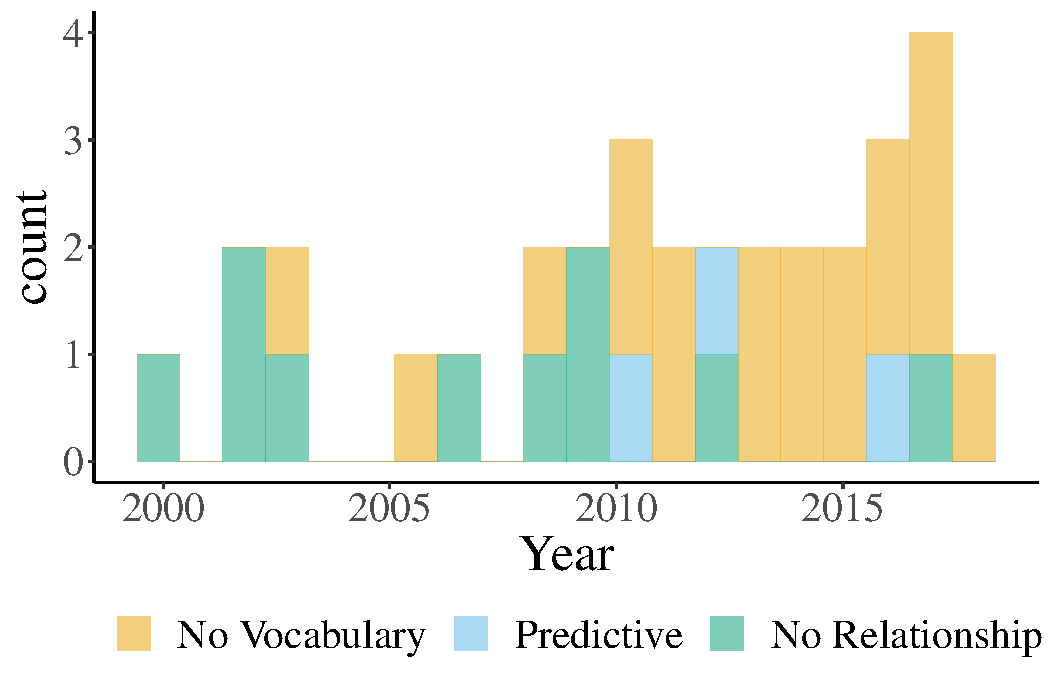
\includegraphics{VonHolzenBergmann_MPMetaAnalysis_files/figure-latex/Vocabdescribe1-1.pdf}
\caption{\label{fig:Vocabdescribe1}Counts of studies included in the meta-analysis as a function of publication year, representing whether the study did not measure vocabulary (yellow), did measure vocabulary and was reported to predict mispronunciation sensitivity (blue), or did measure vocabulary and was reported to not predict mispronunciation sensitivity (pink).}
\end{figure}

\hypertarget{interim-discussion-development-of-infants-mispronunciation-sensitivity}{%
\subsubsection{Interim discussion: Development of infants' mispronunciation sensitivity}\label{interim-discussion-development-of-infants-mispronunciation-sensitivity}}

Although infants consider a mispronunciation to be a better match to the target image than to a distractor image, there was a constant and stable effect of mispronunciation sensitivity across all ages. Furthermore, although we found a relationship between vocabulary size (comprehension) and target looking for correct pronunciations, we found no relationship between vocabulary and target looking for mispronunciations. This may be due to too few studies including reports of vocabulary size and more investigation is needed to draw a firm conclusion. These findings support the arguments set by the early specification hypothesis that infants represent words with phonological detail already at the beginning of the second year of life.

Our power analysis revealed that mispronunciation sensitivity studies typically underpowered, with 54\% power and would need to increase their sample from an average of 24 to 44 infants to achieve 80\% power. While this number does not seem to differ dramatically from the observed sample sizes, the impact of the smaller sample sizes on power is thus substantial and should be kept in mind when planning future studies. Furthermore, many studies in this meta-analysis included further factors to be tested, leading to two-way interactions (age versus mispronunciation sensitivity is a common example), which by some estimates require four times the sample size to detect an effect of similar magnitude as the main effect for both ANOVA (Fleiss, 1986) and mixed-effect-model (Leon \& Heo, 2009) analyses. We thus strongly advocate for a consideration of power and the reported effect sizes to test infants' mispronunciation sensitivity and factors influencing this ability.

The studies examined in this meta-analysis examined mispronunciation sensitivity, but many also included more specific questions aimed at uncovering more detailed phonological processes at play during word recognition. Not only are these questions theoretically interesting, they also have the potential to change the difficulty of a mispronunciation sensitivity experiment. It is possible that the lack of developmental change in mispronunciation sensitivity found by our meta-analysis does not capture a true lack of change, but is instead influenced by differences in the types of tasks given to infants of different ages. We examine this possibility in a set of moderator analyses

\hypertarget{moderator-analyses}{%
\subsection{Moderator Analyses}\label{moderator-analyses}}

If infants' word recognition skills are generally thought to improve with age and vocabulary size, research questions that tap more complex processes may be more likely to be investigated in older infants. In this section, we consider each moderator individually and investigate its influence on mispronunciation sensitivity. For most moderators (except mispronunciation size), we combine the correct and mispronounced datasets and include the moderator of condition, to study mispronunciation sensitivity as opposed to object recognition. To better understand the impact of these moderators on developmental change, we include age as subsequent moderator. Results of the 5 main moderator tests (mispronunciation size, mispronunciation position, mispronunciation type, distractor overlap, distractor familiarity) as well as the individual effects for each moderator interaction are reported in Table 2. The statistic that tests whether a specific moderator explains a significant proportion of variance in the data, QM, was significant for all moderators and subsequent significant interactions of critical terms are interpreted. Finally, we analyze the relationship between infant age and the moderator condition they were tested in using Fisher's exact test, which is more appropriate for small sample sizes (Fisher, 1922). This evaluates the independence of infants' age group (divided into quartiles unless otherwise specified) and assignment to each type of condition in a particular moderator.

(Insert Table 2 about here)

\hypertarget{size-of-mispronunciation}{%
\subsubsection{Size of mispronunciation}\label{size-of-mispronunciation}}

To assess whether the size of the mispronunciation tested, as measured by the number of features changed, modulates mispronunciation sensitivity, we calculated the meta-analytic effect for object identification on a subset of the overall dataset, with 90 records for correct pronunciations, 99 for 1-feature mispronunciations, 16 for 2-feature mispronunciations, and 6 for 3-feature mispronunciations. Each feature change (from 0 to 3; 0 representing correct pronunciations) was considered to have an graded impact on mispronunciation sensitivity (Mani \& Plunkett, 2011; White \& Morgan, 2008) and this moderator was coded as a continuous variable. We did not include records for which the number of features changed was not specified or consistent within a record (e.g., both 1- and 2-feature changes within one mispronunciation record).

\begin{figure}
\centering
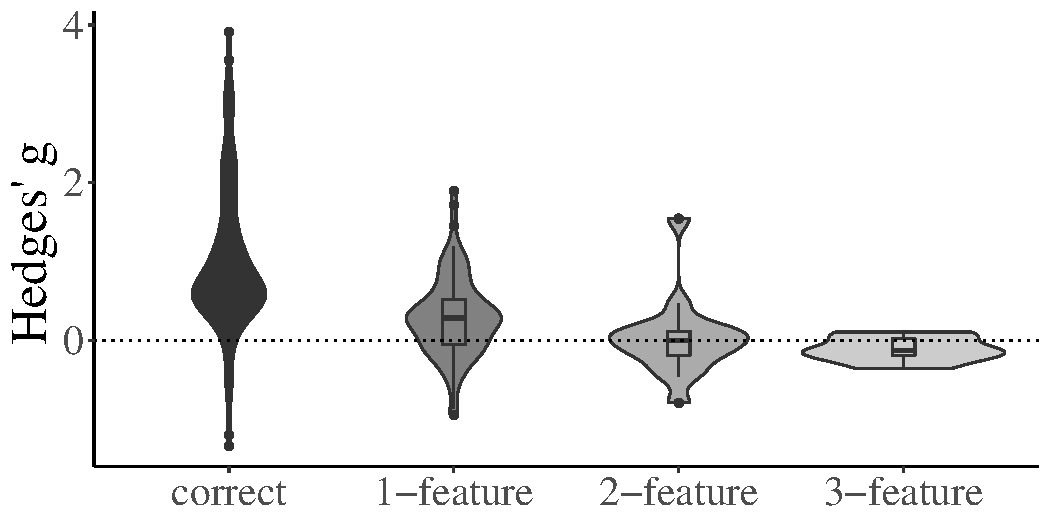
\includegraphics{VonHolzenBergmann_MPMetaAnalysis_files/figure-latex/PlotFeatEffect-1.pdf}
\caption{\label{fig:PlotFeatEffect}Effect sizes for correct pronunciations, 1-, 2-, and 3-feature mispronunciations.}
\end{figure}

The model results revealed that as the number of features changed increased, the effect size Hedges' \emph{g} significantly decreased (Table 2). We plot this relationship in Figure \ref{fig:PlotFeatEffect}. Age did not modulate this effect. Finally, results of Fisher's exact test were not significant, \emph{p} = 0.703.

(Insert Figure \ref{fig:PlotFeatEffect} about here)

\hypertarget{position-of-mispronunciation}{%
\subsubsection{Position of mispronunciation}\label{position-of-mispronunciation}}

We next calculated the meta-analytic effect of mispronunciation sensitivity (moderator: condition) in response to mispronunciations on the onset (\emph{n} = 143 records), medial (\emph{n} = 48), and coda phonemes (\emph{n} = 10). We coded the onset, medial, and coda positions as continuous variables, to evaluate the importance of each subsequent position (Marslen-Wilson \& Zwitserlood, 1989). We did not include data for which the mispronunciation varied within record in regard to position (\emph{n} = 40) or was not reported (\emph{n} = 10).

\begin{figure}
\centering
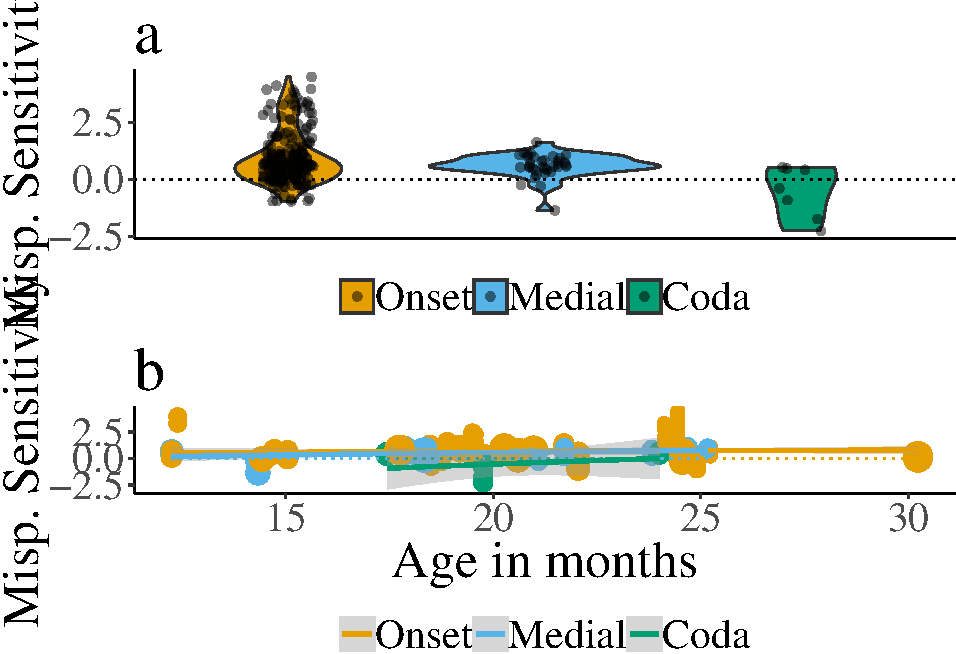
\includegraphics{VonHolzenBergmann_MPMetaAnalysis_files/figure-latex/PlotMispPosit-1.pdf}
\caption{\label{fig:PlotMispPosit}Effect sizes for mispronunciation sensitivity within subject group and study (correct - mispronunciations) for mispronunciations on the onset, medial, and coda positions. The dashed line indicates zero (chance).}
\end{figure}

The model results revealed that mispronunciation sensitivity decreased linearly as the position of the mispronunciation moved later in the word, with sensitivity greatest for onset mispronunciations and smallest for coda mispronunciations (Table 2). We plot this relationship in Figure \ref{fig:PlotMispPosit}. When age was added as a moderator, however, the interaction between age, condition, and mispronunciation position was small and not significant. Due to the small sample size of coda mispronunciations, we only included 3 age groups in Fisher's exact test. The results were significant, \emph{p} = 0.02. Older infants were more likely to be tested on onset mispronunciations, while younger infants were more likely to be tested on medial mispronunciations.

(Insert Figure \ref{fig:PlotMispPosit} about here)

\hypertarget{type-of-mispronunciation-consonant-or-vowel}{%
\subsubsection{Type of mispronunciation (consonant or vowel)}\label{type-of-mispronunciation-consonant-or-vowel}}

We next calculated the meta-analytic effect of mispronunciation sensitivity (moderator: condition) in response to the type of mispronunciation, consonant (\emph{n} = 145) or vowel (\emph{n} = 71). Furthermore, sensitivity to consonant and vowel mispronunciations is hypothesized to differ depending on the language family of the infant's native language. Infants learning American English (\emph{n} = 56), British English (\emph{n} = 66), Danish (\emph{n} = 6), Dutch (\emph{n} = 58), and German (\emph{n} = 21) were classified into the Germanic language family (\emph{n} = 207). Infants learning Catalan (\emph{n} = 4), Spanish (\emph{n} = 4), French (\emph{n} = 8), Catalan and Spanish simultaneously (i.e.~bilinguals; \emph{n} = 6), and Swiss French (\emph{n} = 6) were classified into the Romance language family (\emph{n} = 28). We therefore conducted two sets of analyses, one analyzing consonants and vowels alone and a second including langauge family (Germanic vs.~Romance) as a moderator. We did not include data for which mispronunciation type varied within experiment and was not reported separately (\emph{n} = 23).

\begin{figure}
\centering
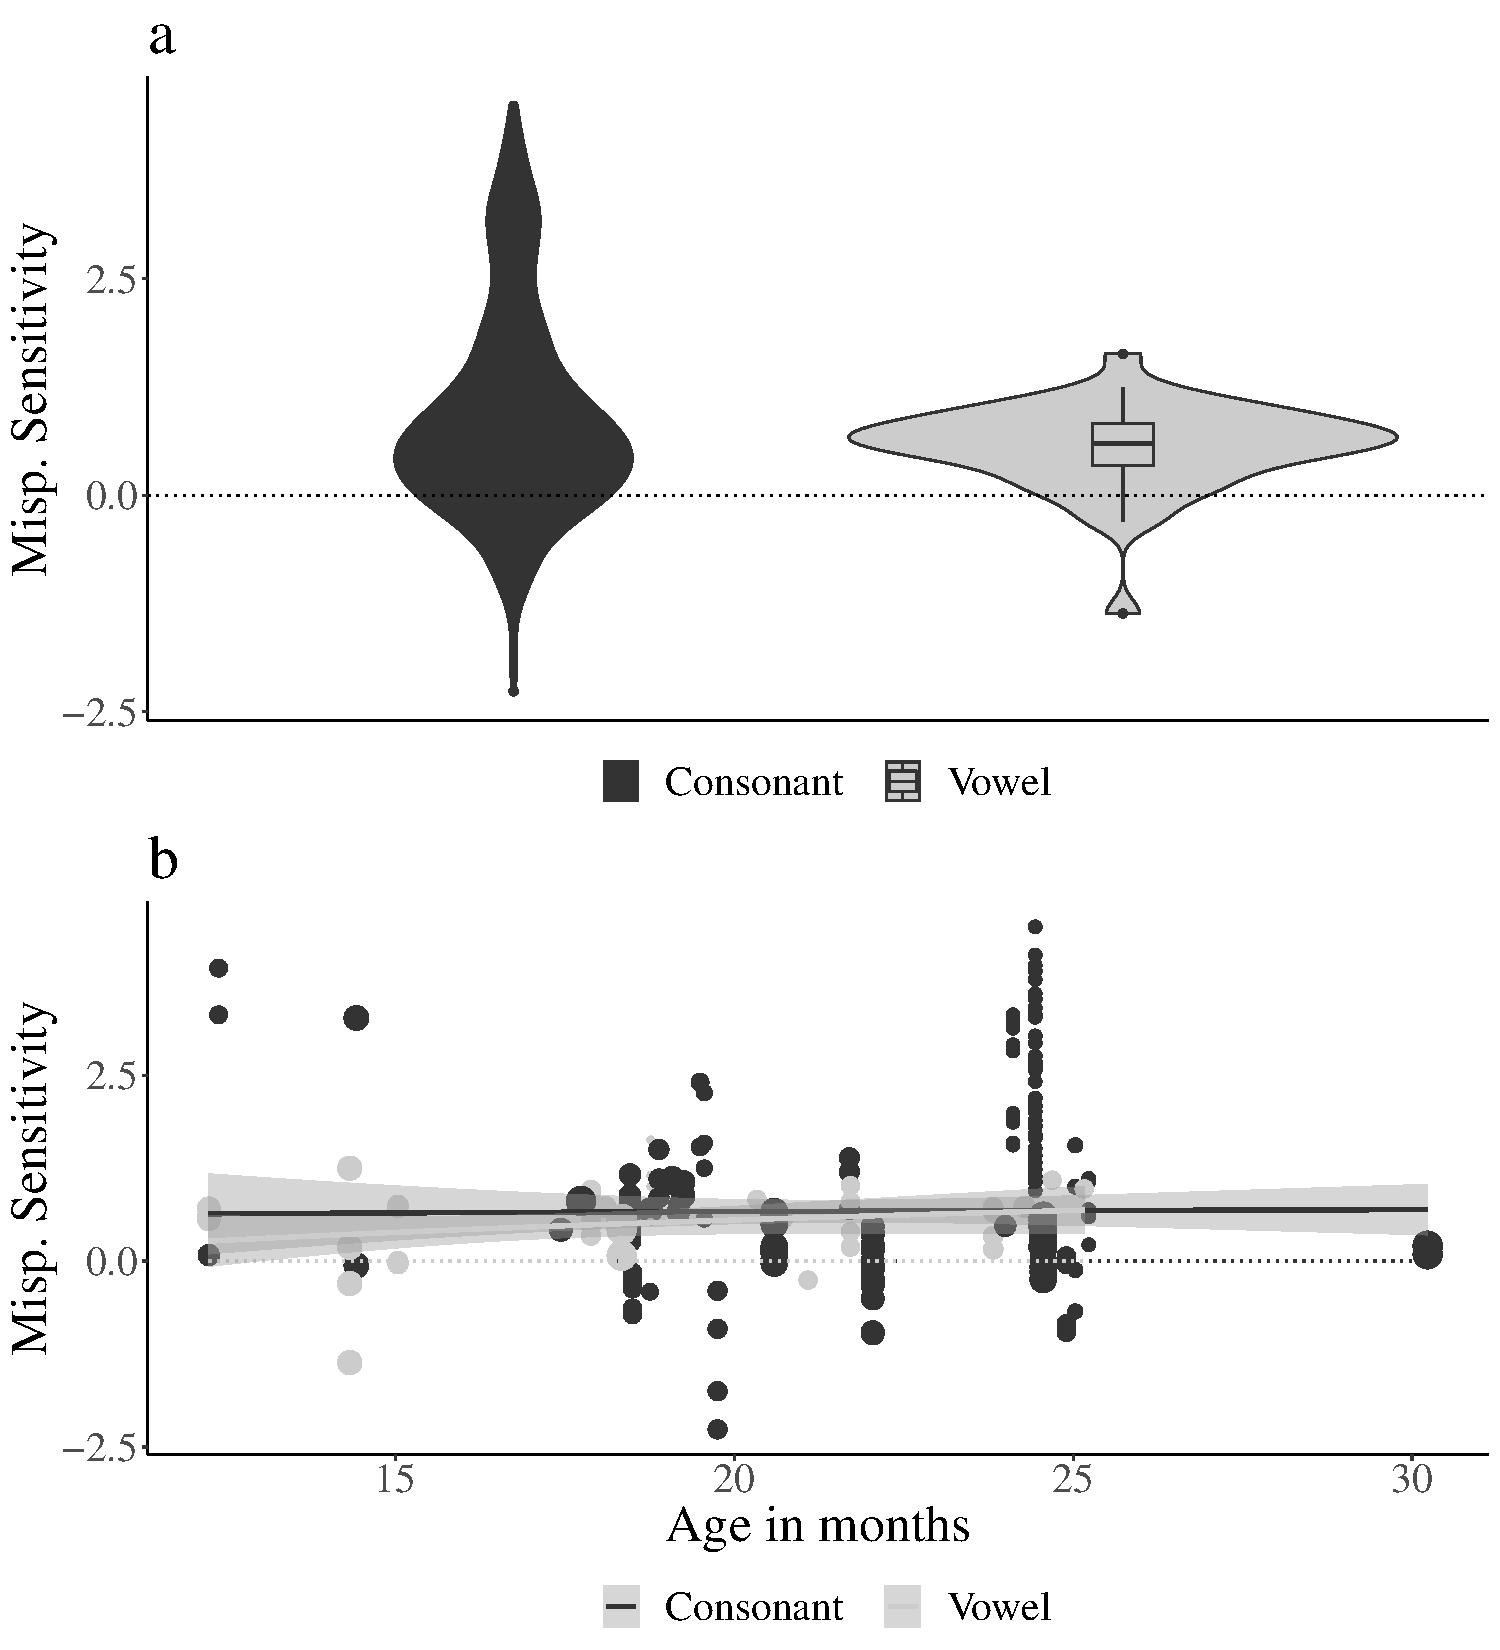
\includegraphics{VonHolzenBergmann_MPMetaAnalysis_files/figure-latex/PlotMispType-1.pdf}
\caption{\label{fig:PlotMispType}Panel a: Effect sizes for mispronunciation sensitivity within subject group and study (correct - mispronunciations) for consonant and vowel mispronunciations. Panel b: Effect sizes for mispronunciation sensitivity within subject group and study (correct - mispronunciations) for consonant and vowel mispronunciations by age. For both panels, point size depicts inverse variance and the dashed line indicates zero (chance).}
\end{figure}

The model results revealed that mispronunciation sensitivity did not differ between consonant and vowel mispronunciations (Table 2). We plot this relationship in Figure \ref{fig:PlotMispType}a. When age was added as a moderator, however, the model revealed that as infants age, mispronunciation sensitivity grows larger for vowel mispronunciations but stays steady for consonant mispronunciations (Figure \ref{fig:PlotMispType}b). The results of Fisher's exact test were significant, \emph{p} \textless{} .001. Older infants were more likely to be tested on consonant mispronunciations, while younger infants were more likely to be tested on vowel mispronunciations. Whether consonant or vowel mispronunciations are more ``difficult'' is a matter of theoretical debate, but some evidence suggest that it may be influenced by infants' native language (Nazzi et al., 2016). We next examined whether this was the case.

(Insert Figure \ref{fig:PlotMispType} about here)

\begin{figure}
\centering
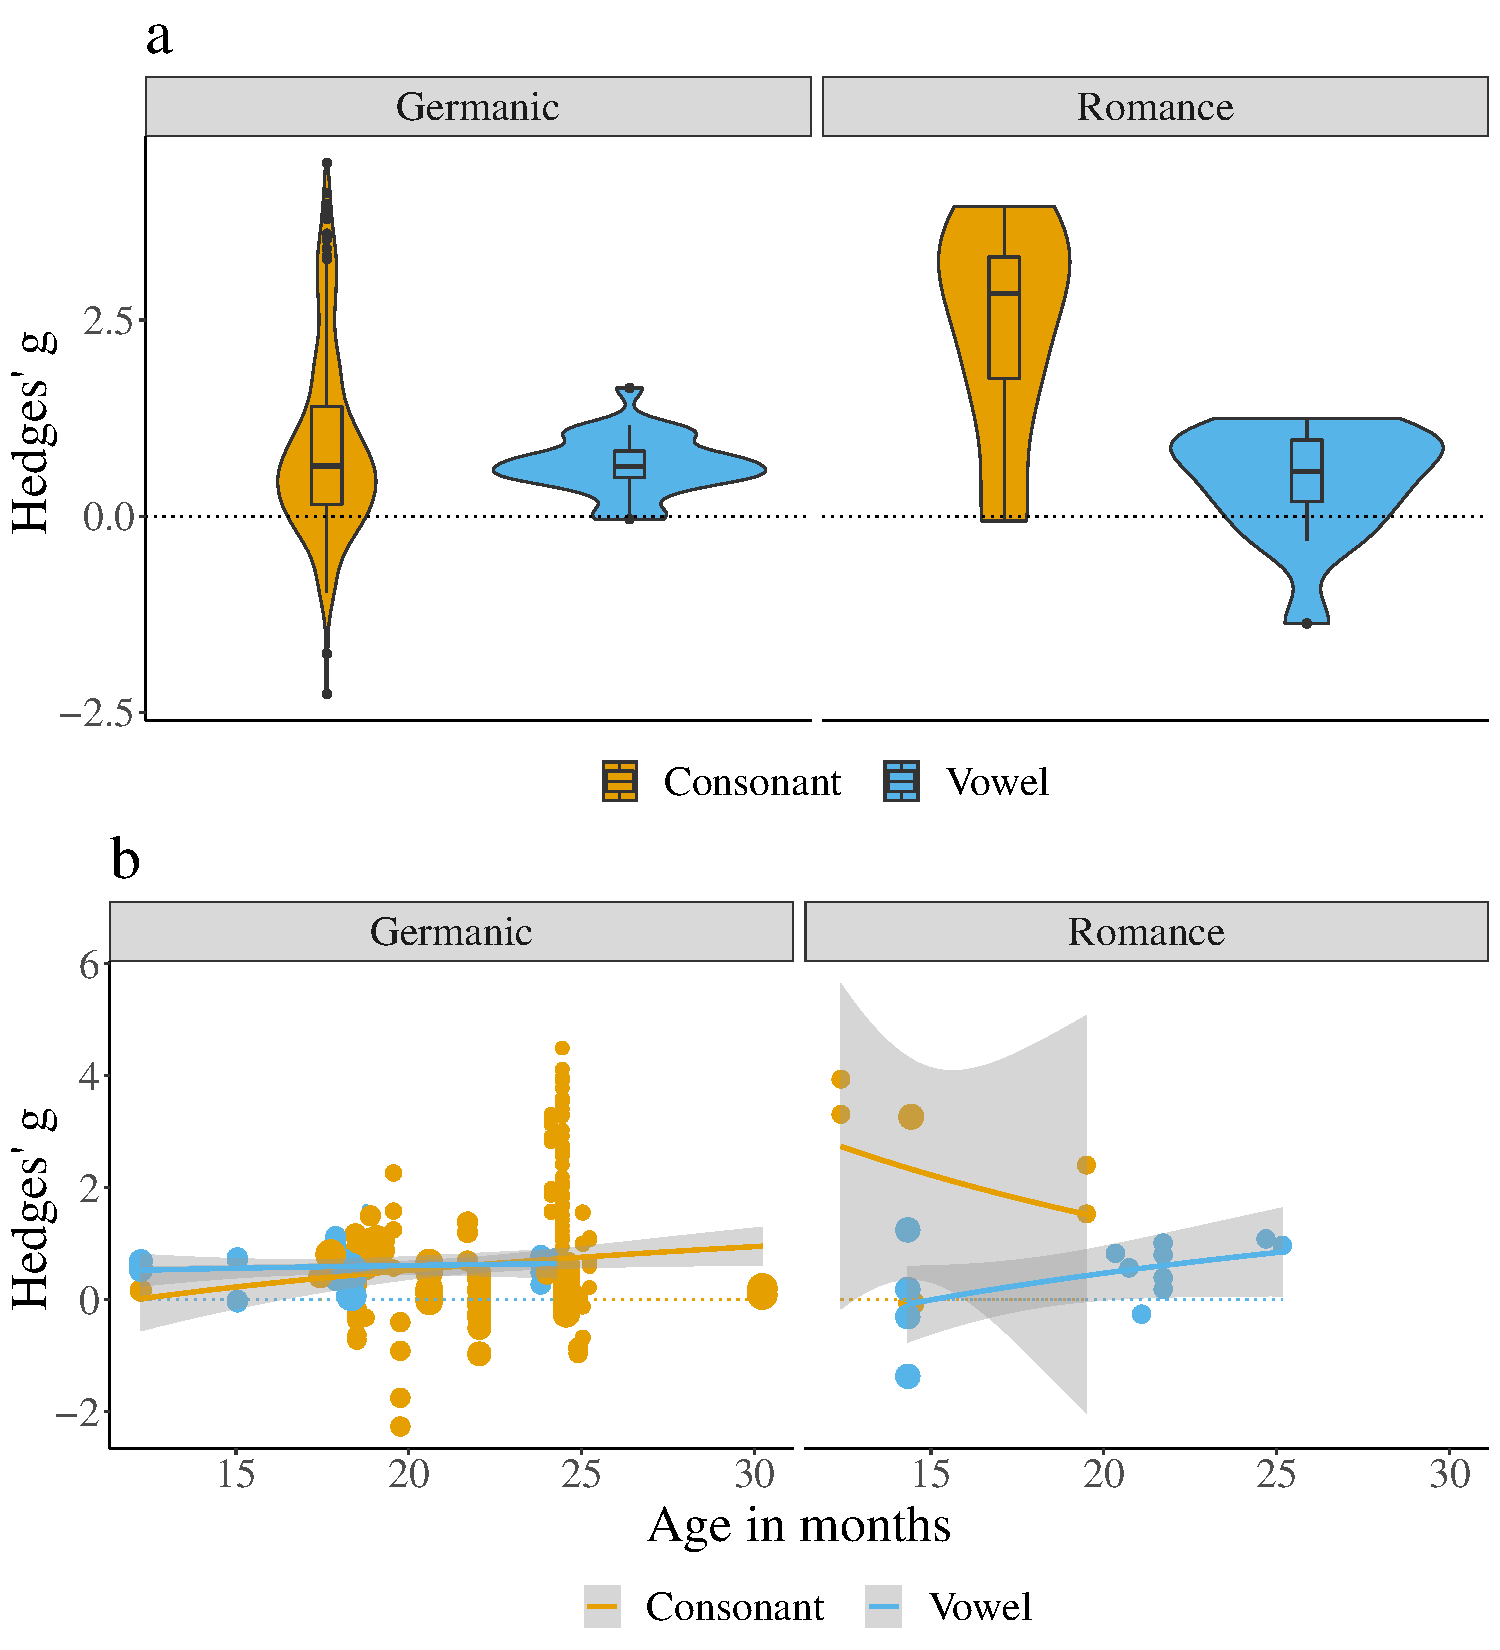
\includegraphics{VonHolzenBergmann_MPMetaAnalysis_files/figure-latex/PlotCVEffectLang-1.pdf}
\caption{\label{fig:PlotCVEffectLang}Panel a: Effect sizes for mispronunciation sensitivity within subject group and study (correct - mispronunciations) for consonant and vowel mispronunciations for infants learning a Germanic (left) or a Romance (right) native language. Panel b: Effect sizes for mispronunciation sensitivity within subject group and study (correct - mispronunciations) for consonant and vowel mispronunciations for infants learning a Germanic (left) or a Romance (right) native language by age. For both panels, point size depicts inverse variance and the dashed line indicates zero (chance).}
\end{figure}

The model results revealed that mispronunciation sensitivity for consonants was similar for Germanic and Romance languages. Mispronunciation sensitivity for vowels, however, was greater for Germanic compared to Romance languages (Table 2). We plot this relationship in Figure \ref{fig:PlotCVEffectLang}a. Adding age as a moderator revealed a small but significant estimate for the four-way interaction between mispronunciation type, condition, language family, and age. As can also be seen in Figure \ref{fig:PlotCVEffectLang}b, for infants learning Germanic languages, sensitivity to consonant and vowel mispronunciations did not change with age. In contrast, infants learning Romance languages show a decrease in sensitivity to consonant mispronunciations, but an increase in sensitivity to vowel mispronunciations with age. Due to the small sample size of infants learning Romance languages, we were unable to use Fisher's exact test.

(Insert Figure \ref{fig:PlotCVEffectLang} about here)

\hypertarget{phonological-overlap-between-target-and-distractor}{%
\subsubsection{Phonological overlap between target and distractor}\label{phonological-overlap-between-target-and-distractor}}

We next examined the meta-analytic effect of mispronunciation sensitivity (moderator: condition) in response to mispronunciations when the target-distractor pairs either had no overlap (\emph{n} = 80) or shared the same onset phoneme (\emph{n} = 104). We did not include data for which the overlap included other phonemes (i.e.~onset and medial, coda) or the distractor was an unfamiliar object.

\begin{figure}
\centering
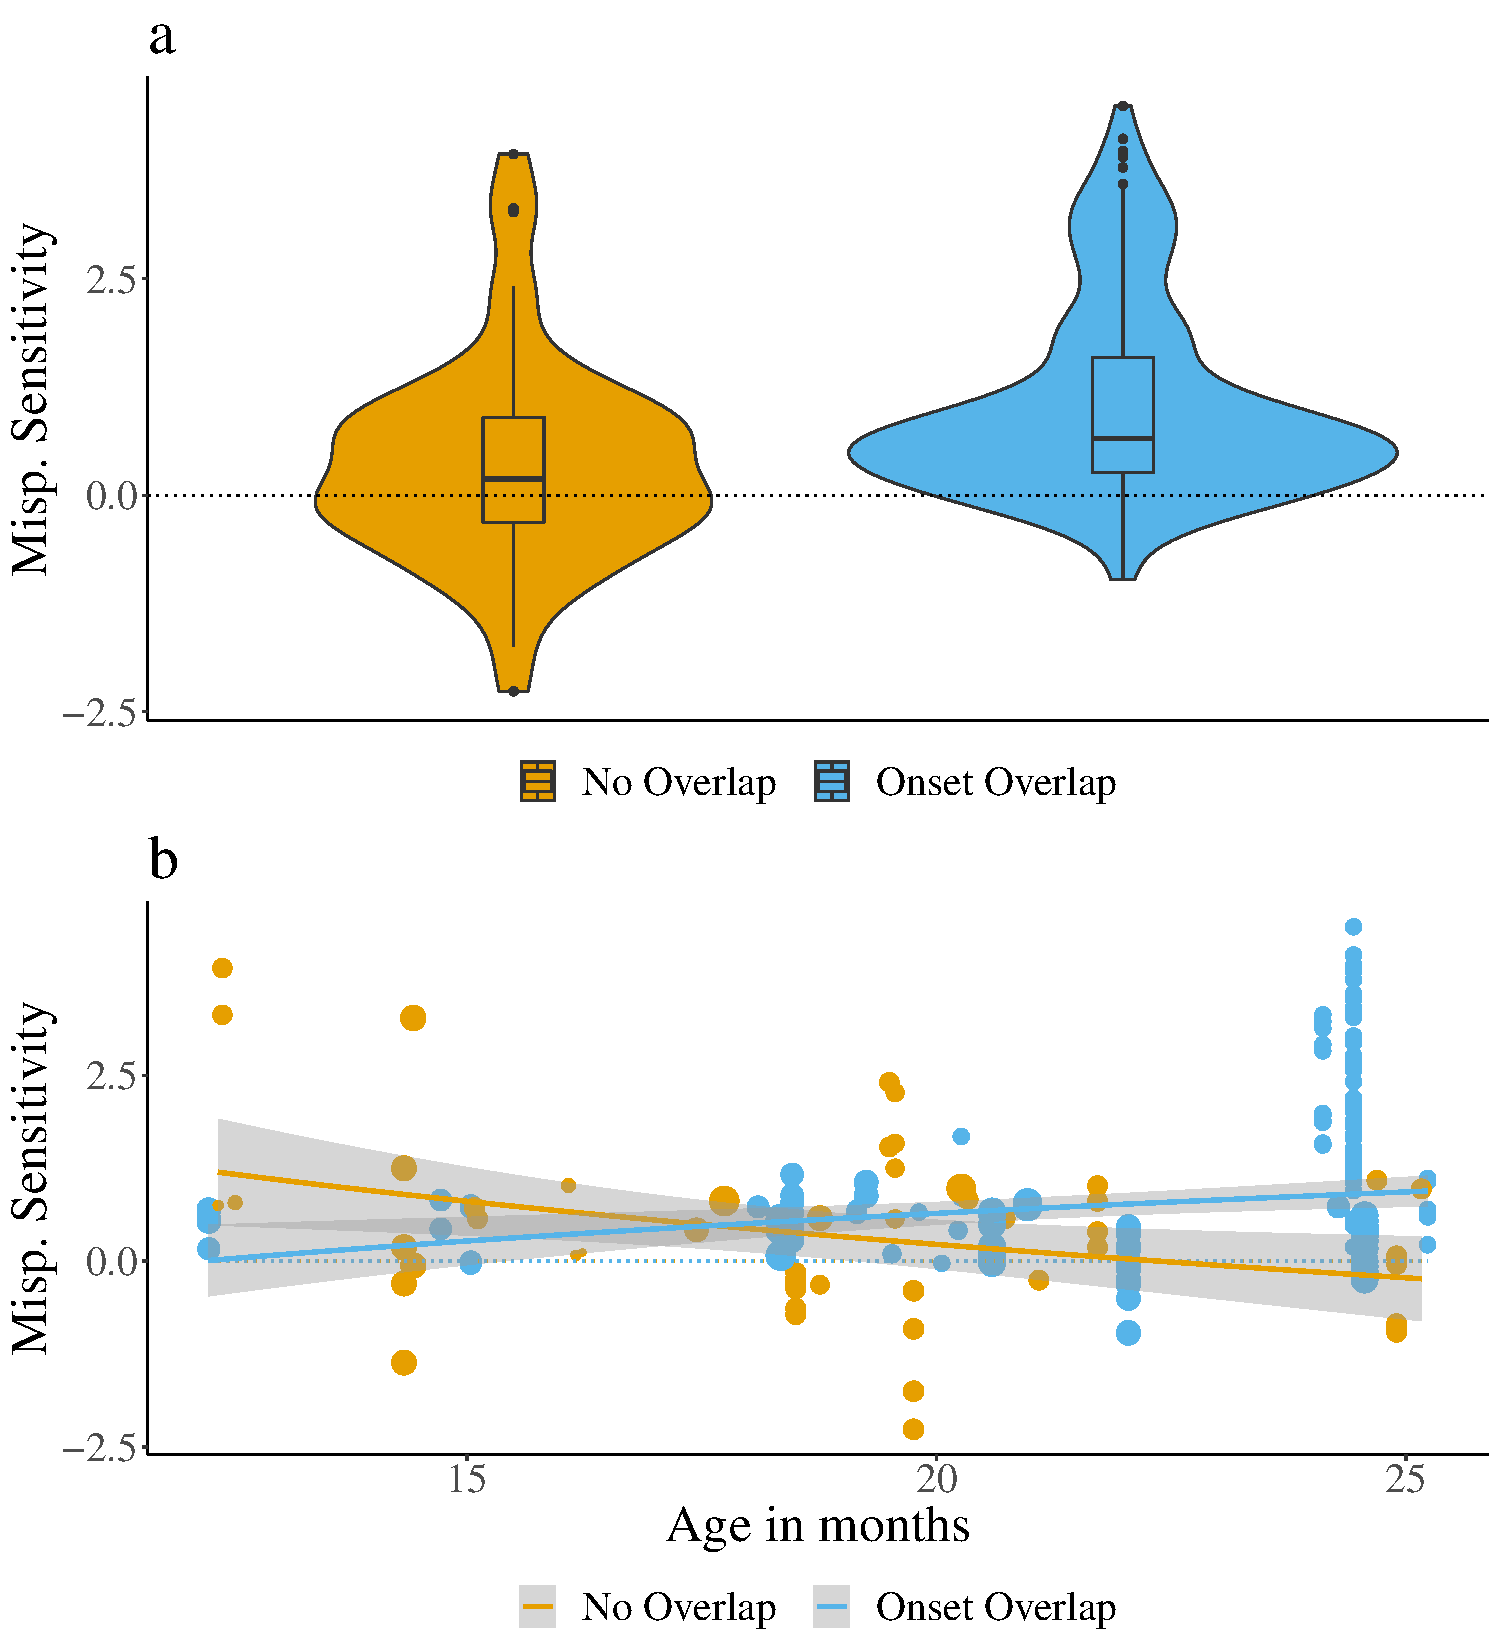
\includegraphics{VonHolzenBergmann_MPMetaAnalysis_files/figure-latex/PlotDistOverlap-1.pdf}
\caption{\label{fig:PlotDistOverlap}Panel a: Effect sizes for mispronunciation sensitivity within subject group and study (correct - mispronunciations) for target-distractor pairs with onset overlap or no overlap. Panel b: Effect sizes for mispronunciation sensitivity within subject group and study (correct - mispronunciations) for target-distractor pairs with onset overlap or no overlap by age. For both panels, point size depicts inverse variance and the dashed line indicates zero (chance).}
\end{figure}

The model results revealed that mispronunciation sensitivity was greater when target-distractor pairs shared the same onset phoneme compared to when they shared no phonological overlap (Table 2). We plot this relationship in Figure \ref{fig:PlotDistOverlap}a. Adding age as a moderator revealed a small but significant estimate for the three-way interaction between age, condition, and distractor overlap (Figure \ref{fig:PlotCVEffectLang}b). Mispronunciation sensitivity increased with age for target-distractor pairs containing onset overlap, but decreased with age for target-distractor pairs containing no overlap. The results of Fisher's exact test were significant, \emph{p} \textless{} .001. Older infants were more likely to be tested in experimental conditions where target and distractor images overlapped on their onset phoneme, while younger infants were more likely to be tested in experimental conditions that did not control for overlap.

(Insert Figure \ref{fig:PlotDistOverlap} about here)

\hypertarget{distractor-familiarity}{%
\subsubsection{Distractor familiarity}\label{distractor-familiarity}}

We next calculated the meta-analytic effect of mispronunciation sensitivity (moderator: condition) in experiments were the target image was paired with a familiar (\emph{n} = 179) or unfamiliar (\emph{n} = 72) distractor image.

\begin{lltable}

\scriptsize{

\begin{longtable}{lllllll}\noalign{\getlongtablewidth\global\LTcapwidth=\longtablewidth}
\caption{\label{tab:mod_table_finalize}Summary of the 5 moderator tests, including effect estimates for effects and critical interactions.}\\
\toprule
Moderator & Moderator Test & Interaction Terms & Hedges' *g* & SE & 95 CI & *p*-value\\
\midrule
\endfirsthead
\caption*{\normalfont{Table \ref{tab:mod_table_finalize} continued}}\\
\toprule
Moderator & Moderator Test & Interaction Terms & Hedges' *g* & SE & 95 CI & *p*-value\\
\midrule
\endhead
Misp. size & QM(1) = 59.618, *p* < .001 &  & -0.403 & 0.052 & [-0.505, -0.301] & < .001\\
 & QM(3) = 140.626, *p* < .001 & Age & 0.009 & 0.006 & [-0.002, 0.02] & = 0.099\\ \midrule
Misp. position & QM(3) = 172.935, *p* < .001 & Condition & -0.146 & 0.064 & [-0.271, -0.02] & = 0.023\\
 & QM(7) = 176.208, *p* < .001 & Condition * Age & 0.018 & 0.018 & [-0.017, 0.053] & = 0.314\\ \midrule
Misp. type & QM(3) = 141.83, *p* < .001 & Condition & 0.043 & 0.079 & [-0.111, 0.198] & = 0.584\\
 & QM(7) = 149.507, *p* < .001 & Condition * Age & 0.041 & 0.018 & [0.005, 0.076] & = 0.026\\
 & QM(7) = 154.731, *p* < .001 & Condition * Language Family & -0.841 & 0.28 & [-1.39, -0.292] & = 0.003\\
 & QM(15) = 181.174, *p* < .001 & Condition * Language Family * Age & 0.344 & 0.078 & [0.191, 0.496] & < .001\\ \midrule
Distractor overlap & QM(3) = 48.551, *p* < .001 & Condition & 0.199 & 0.215 & [-0.222, 0.619] & = 0.354\\
 & QM(7) = 68.485, *p* < .001 & Condition * Age & 0.092 & 0.038 & [0.017, 0.166] & = 0.016\\ \midrule
Distractor familiarity & QM(3) = 102.487, *p* < .001 & Condition & 0.038 & 0.138 & [-0.233, 0.309] & = 0.783\\
 & QM(7) = 106.262, *p* < .001 & Condition * Age & -0.02 & 0.035 & [-0.089, 0.049] & = 0.574\\
\bottomrule
\end{longtable}

}

\end{lltable}

The model results revealed that infants' familiarity with the distractor object (familiar or unfamiliar) did not impact their mispronunciation sensitivity, nor was this relationship influenced by the age of the infant. The results of Fisher's exact test were not significant, \emph{p} = 0.072.

\hypertarget{interim-discussion-moderator-analyses}{%
\subsubsection{Interim discussion: Moderator analyses}\label{interim-discussion-moderator-analyses}}

Mispronunciation sensitivity was modulated overall by the size of the mispronunciation tested, whether target-distractor pairs shared phonological overlap, and the position of the mispronunciation. Neither distractor familiarity (familiar, unfamiliar) or type of mispronunciation (consonant, vowel) were found to impact mispronunciation sensitivity.

When age was added as a moderator, mispronunciation sensitivity was found to vary by type of mispronunciation and overlap between the target and distractor labels over development, but age did not influence sensitivity to mispronunciation size, mispronunciation position, and distractor familiarity. Finally, in some cases there was evidence that older and younger infants were given experimental manipulations that may have rendered the experimental task more or less difficult. In one instance, younger infants were given a more difficult task, mispronunciations on the medial position, which is unlikely to contribute to the lack of developmental effects in our main analysis. Yet, this was not always the case; in a different instance, older children were more likely to be given target-distractor pairs that overlapped on their onset phoneme, a situation in which it is more difficult to detect a mispronunciation and may have bearing on our main developmental results. We return to these findings in the General Discussion.

\hypertarget{exploratory-analyses}{%
\subsection{Exploratory Analyses}\label{exploratory-analyses}}

We next considered whether an effect of maturation might have been masked by other factors we have not yet captured in our analyses. A strong candidate that emerged during the construction of the present dataset and careful reading of the original papers was the analysis approach. We observed, as mentioned in the Methods section, variation in the dependent variable reported, and additionally noted that the size of the chosen post-naming analysis window varied substantially across papers. Researchers' analysis strategy may be adapted to infants' age or influenced by having observed the data. For example, consider the possibility that a particular study does not find that infants looked to the target object upon hearing a correct pronunciation. With this pattern of behavior, interpreting an effect of mispronunciation sensitivity becomes difficult; how can infants notice a phoneme change when they do not even show recognition of the correct pronunciation? A lack of recognition or a small effect for correct pronunciations would be more difficult to publish (Ferguson \& Heene, 2012). In order to have publishable results, adjustments to the analysis approach could be made until a significant effect of recognition for correct pronunciations is found. But, these adjustments would also need to be made for the analysis of mispronunciations, which may impact the size of the mispronunciation sensitivity effect. Such a scenario could explain the publication bias suggested by the asymmetry for correct pronunciations in the funnel plot shown in Figure \ref{fig:FunnelCombo} (Simmons, Nelson, \& Simonsohn, 2011). This could lead to an increase in significant results and even alter the apparent developmental trajectory of mispronunciation sensitivity measured in experiments.

We examine whether variation in the approach to data analysis may be have an influence on our conclusions regarding infants' developing mispronunciation sensitivity. To do so, we analyzed analysis choices related to timing, specifically the post-naming analysis window, as well as type of dependent variable in our coding of the dataset because they are consistently reported. Further, since we observe variation in both aspects of data analysis, summarizing typical choices and their impact might be useful for experiment design in the future and might help establish field standards. In the following, we discuss the possible theoretical motivation for these data analysis choices, the variation present in the current meta-analysis dataset, and the influence these analysis choices may have on reported mispronunciation sensitivity and its development. We focus specifically on the size of the mispronunciation sensitivity effect, considering the whole dataset and including condition (correct pronunciation, mispronunciation) as a moderator.

\hypertarget{timing}{%
\subsubsection{Timing}\label{timing}}

When designing mispronunciation sensitivity studies, experimenters can choose the length of time each trial is presented. This includes both the length of time before the target object is named (pre-naming phase) as well as after (post-naming phase) and is determined prior to data collection. Evidence suggests that the speed of word recognition is slower in young infants (Fernald et al., 1998), which may lead researchers to include longer post-naming phases in their experiments with younger infants. The post-naming analysis window, in contrast, represents how much of this phase was included in the statistical analysis and can be chosen after the experimental data is collected and perhaps observed. If infant age is influencing the length of these windows, we should expect a negative correlation.

Across papers, there was wide variation in the length of the post-naming phase (\emph{Median} = 3500 ms, range = 2000 - 9000) and the post-naming analysis window (\emph{Median} = 2500 ms, range = 1510 - 4000). The most popular post-naming phase length was 4000 ms (\emph{n} = 74 records) and 2000 ms (\emph{n} = 97 records) was the most popular for the post-naming analysis window. About half of the records were analyzed using the whole post-naming phase presented to the infant (\emph{n} = 124), while the other half were analyzed using a shorter portion of the post-naming time window, usually excluding later portions (\emph{n} = 127).

There was no apparent relation between infant age and post-naming phase length (\emph{r} = 0.01, 95\% CI{[}-0.11, 0.13{]}, \emph{p} = 0.882), but there was a significant negative relationship between infant age and post-naming analysis window length, such that younger infants' looking times were analyzed using a longer post-naming analysis window (\emph{r} = -0.23, 95\% CI{[}-0.35, -0.11{]}, \emph{p} \textless{} .001). We next investigated whether post-naming analysis window length impacted measures of mispronunciation sensitivity.

\begin{figure}
\centering
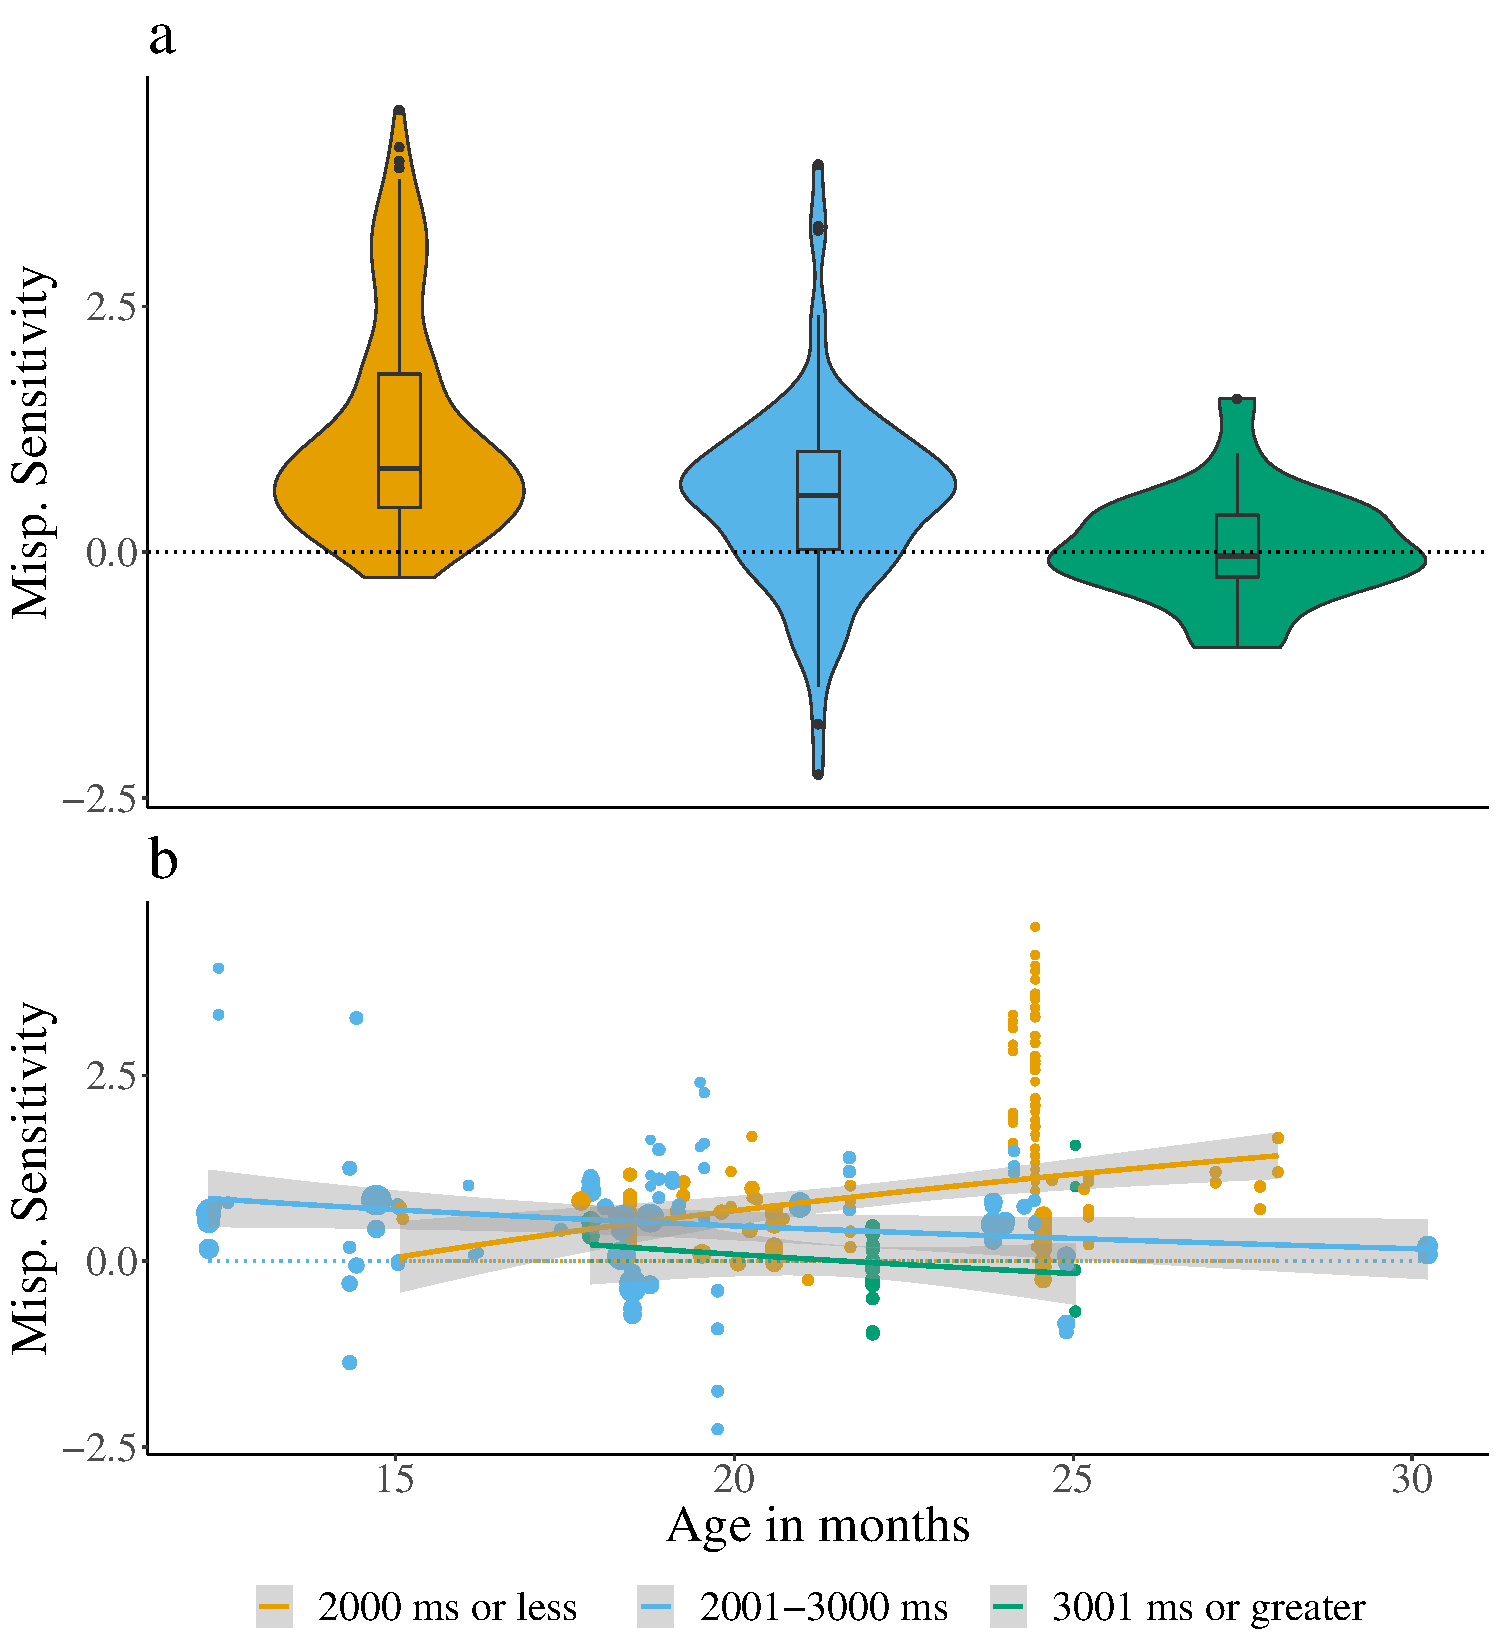
\includegraphics{VonHolzenBergmann_MPMetaAnalysis_files/figure-latex/PlotPostNameCondAge-1.pdf}
\caption{\label{fig:PlotPostNameCondAge}Effect sizes for the different lengths of the post-naming analysis window: 2000 ms or less (yellow), 2001 to 3000 ms (blue), and 3001 ms or greater (pink). Although length of the post-naming analysis window was included as a continuous variable in the meta-analytic model, it is divided into categories for ease of viewing. Panel a plots mispronunciation sensitivity aggregated over age, while panel b plots mispronunciation sensitivity, within subject group and study (correct - mispronunciations), as a function of age. The lines plot the linear regression and the gray shaded area indicates the standard error.}
\end{figure}

When post-naming analysis window length and condition (correct pronunciation, mispronunciation) were included as moderators, the moderator test was significant (QM(3) = 237.055, \emph{p} \textless{} .001). The estimate for the interaction between post-naming analysis window and condition was small but significant (\(\beta\) = -0.268, SE = 0.059, 95\% CI{[}-0.383, -0.153{]}, \emph{p} \textless{} .001), showing that as the length of the post-naming analysis window increased, the difference between target fixations for correctly pronounced and mispronounced items (mispronunciation sensitivity) decreased. This relationship is plotted in Figure \ref{fig:PlotPostNameCondAge}a. When age was added as a moderator, the moderator test was significant (QM(7) = 247.485, \emph{p} \textless{} .001). The estimate for the three-way-interaction between condition, post-naming analysis window, and age was small, but significant (\(\beta\) = -0.04, SE = 0.014, 95\% CI{[}-0.068, -0.012{]}, \emph{p} = 0.006). As can be seen in Figure \ref{fig:PlotPostNameCondAge}b, when records were analyzed with a post-naming analysis window of 2000 ms or less (a limit we imposed for visualization purposes), mispronunciation sensitivity seems to increase with infant age. If the post-naming analysis window is greater than 2000 ms, however, there is no or a negative relation between mispronunciation sensitivity and age.

(Insert Figure \ref{fig:PlotPostNameCondAge} about here)

\hypertarget{dependent-variable}{%
\subsection{Dependent variable}\label{dependent-variable}}

As described in the Methods section, there was considerable variation across papers in whether the pre-naming phase was used as a baseline measurement (Difference Score or Pre- vs.~Post) or whether the post-naming PTL was compared with a chance value of 50\% (Post). Considering analyses of the dependent variables Difference Score or Pre- vs.~Post produce the same result, we combined these two dependent variables into one, which we call Baseline Corrected. To our knowledge, there is no theory or evidence that explicitly drives choice of dependent variable in preferential looking studies, which may explain the wide variation in dependent variable reported in the papers included in this meta-analysis. We next explored whether the type of dependent variable calculated was related to the estimated size of sensitivity to mispronunciations.

\begin{figure}
\centering
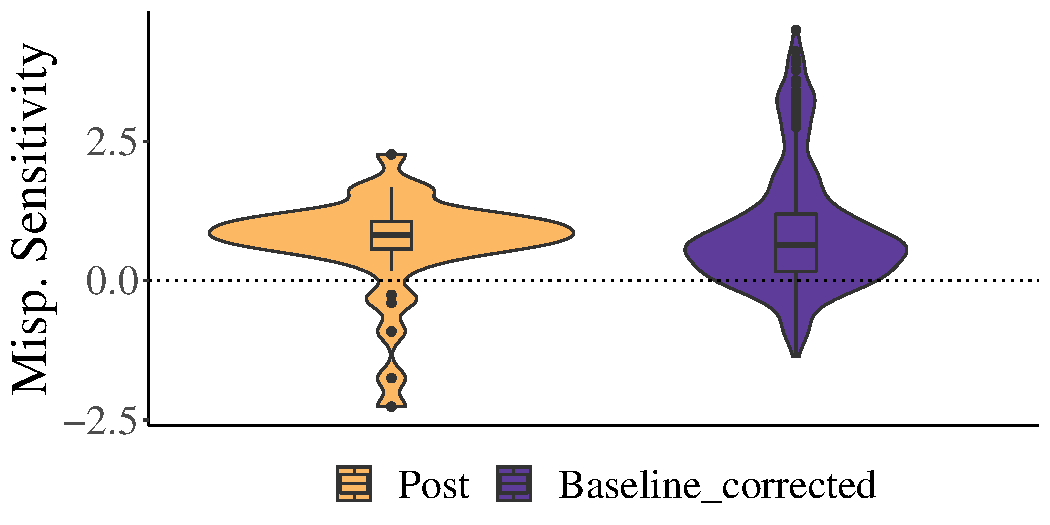
\includegraphics{VonHolzenBergmann_MPMetaAnalysis_files/figure-latex/PlotWithinCondDVbaseline-1.pdf}
\caption{\label{fig:PlotWithinCondDVbaseline}Effect sizes for the different types of dependent variables calculated: Post (yellow), Post vs.~Pre (blue), and Difference Score (pink). Panel a plots mispronunciation sensitivity aggregated over age, while panel b plots mispronunciation sensitivity, within subject group and study (correct - mispronunciations), as a function of age. The lines plot the linear regression and the gray shaded area indicates the standard error.}
\end{figure}

When we included both condition and dependent variable as moderators, the moderator test was significant (QM(3) = 231.004, \emph{p} \textless{} .001). The estimate for the interaction between the type of dependent variable and condition was was significant (\(\beta\) = -0.185, SE = 0.093, 95\% CI{[}-0.366, -0.003{]}, \emph{p} = 0.046). As can be seen in \ref{fig:PlotWithinCondDVbaseline}, mispronunciation sensitivity was higher when the dependent variable reported was Post compared to when it was Baseline Corrected. When age was included as an additional moderator, the moderator test was significant (QM(7) = 237.51, \emph{p} \textless{} .001). However, the estimate for the interaction between dependent variable, condition, and age was not significant (\(\beta\) = -0.049, SE = 0.026, 95\% CI{[}-0.1, 0.002{]}, \emph{p} = 0.061).

(Insert Figure \ref{fig:PlotWithinCondDVbaseline} about here)

\hypertarget{general-discussion}{%
\section{General Discussion}\label{general-discussion}}

In this meta-analysis, we set out to quantify and assess the phonological specificity of infants' representations for familiar words and how this is modulated with development, as measured by infant age and vocabulary size. Infants not only recognize object labels when they were correctly pronounced, but are also likely to accept mispronunciations as labels for targets. Nonetheless, there was a considerable difference in target fixations in response to correctly pronounced and mispronounced labels, suggesting that infants show sensitivity to what constitutes unacceptable, possibly meaning-altering variation in word forms, thereby displaying knowledge of the role of phonemic changes throughout the ages assessed here (6 to 30 months). At the same time, infants, like adults, can recover from mispronunciations, a key skill in language processing.

Considering the variation in findings of developmental change in mispronunciation sensitivity (see Introduction), we next evaluated the developmental trajectory of infants' mispronunciation sensitivity. Our analysis of this relationship revealed a pattern of unchanging sensitivity over infant age and vocabulary size, which has been reported by a handful of studies directly comparing infants over a small range of ages, such as 18-24 months (Bailey \& Plunkett, 2002; Swingley \& Aslin, 2000) or 12-17 months (Zesiger et al., 2012). The lack of age or vocabulary effects in our meta-analysis suggest that this understanding is present from an early age and is maintained throughout early lexical development. We note, however, that despite an increasing publication record of mispronunciation sensitivity studies, fewer than half of the papers included in this meta-analysis measured vocabulary (\emph{n} = 13; out of 32 papers total; see also Figure \ref{fig:Vocabdescribe1}). On the one hand, this may reflect a decreasing interest in the relationship between mispronunciation sensitivity and vocabulary size and/or to invest in data collection that is not expected to yield significant outcomes. On the other hand, non-significant correlations between mispronunciation sensitivity and vocabulary size may be more likely to not be reported, reducing our ability to uncover the true relationship (Rosenthal, 1979; Simonsohn et al., 2014). Considering the theoretical implications, however, more experimental work investigating and reporting the relationship between mispronunciation sensitivity and vocabulary size, whether the relationship is significant or not, is needed if this link is to be evaluated. We encourage researchers to measure and report infants' vocabulary size in future studies. Nonetheless, if we are to take our results as robust, it becomes thus a pressing open question that theories have to answer which other factors might prompt acquiring and using language-specific phonological contrasts at such an early age.

\hypertarget{moderator-analyses-1}{%
\subsection{Moderator Analyses}\label{moderator-analyses-1}}

With perhaps a few exceptions, the main focus of many of the experiments included in this meta-analysis was not to evaluate whether infants are sensitive to mispronunciations in general but rather to investigate specific questions related to phonological and lexical processing and development. We included a set of moderator analyses to better understand these issues by themselves, as well as how they may have impacted our main investigation of infants' development of mispronunciation sensitivity. Several of these moderators include manipulations that make mispronunciation detection more or less difficult for the infant. As a result, the size of the mispronunciation sensitivity effect may be influenced by the task, especially if older infants are given more demanding tasks in comparison to younger infants, potentially masking developmental effects. Considering this, we also evaluated whether the investigation of each of these manipulations was distributed evenly across infant ages, where an uneven distribution may have subsequently heightened or dampened our estimate of developmental change.

The results of the moderator analysis reflect several findings reported in the literature. The meta-analytic effect for mispronunciation size, as measured by phonological features changed, showed graded sensitivity (Bernier \& White, 2017; Mani \& Plunkett, 2011; Tamasi, 2016; White \& Morgan, 2008), an adult-like ability. More studies are needed to evaluate whether this gradual sensitivity develops with age, as only one study examined more than one age (Mani \& Plunkett, 2011) and all others test the same age with a varying number of features (Bernier \& White, 2017; Tamasi, 2016; White \& Morgan, 2008). With more studies investigating graded sensitivity at multiple ages with all other factors held constant, we would achieve a better estimate of whether this is a stable or developing ability, thus also shedding more light on the progression of phono-lexical development in general that then needs to be captured in theories and models.

Our meta-analysis showed that infants are more sensitive to changes in the sounds of familiar words when they occur in an earlier position as opposed to a late position. This awards support to lexical access theories that place greater importance on the onset position during word recognition (i.e.~COHORT; Marslen-Wilson \& Zwitserlood, 1989). At face value, our results thus support theories placing more importance on earlier phonemes. But studies that have contrasted mispronunciations on different positions have found this does not modulate sensitivity (Swingley, 2009; Zesiger et al., 2012). One potential explanation is how the timing of different mispronunciation locations are considered in analysis. For example, Swingley (2009) adjusted the post-naming analysis window start from 367 ms for onset mispronunciations to 1133 for coda mispronunciations, to ensure that infants have a similar amount of time to respond to the mispronunciation, regardless of position. The length of the post-naming analysis window does impact mispronunciation sensitivity, as we discuss below, and mispronunciations that occur later in the word (i.e.~medial and coda mispronunciations) may be at a disadvantage relative to onset mispronunciations if this is not taken into account. These issues can be addressed with the addition of more experiments that directly compare sensitivity to mispronunciations of different positions, as well as the use of analyses that account for timing differences.

For several moderators, we found no evidence of significant modulation of mispronunciation sensitivity. Studies that include an unfamiliar, as opposed to familiar distractor image, often argue that the unfamiliar image provides a better referent candidate for mispronunciation than a familiar distractor image, where the name is already known. Yet, no studies have directly examined this assertion and our meta-analysis found that distractor familiarity did not significantly modulate mispronunciation sensitivity. One possible explanation is that when the size of the mispronunciation is small (e.g.~1-feature change), infants are unlikely to map this label onto a novel object (for evidence from infant word learning see Dautriche, Swingley, \& Christophe, 2015; Swingley, 2016; Swingley \& Aslin, 2007).

Despite the proposal that infants should be more sensitive to consonant compared to vowel mispronunciations (Nazzi et al., 2016), we found no difference in sensitivity to consonant and vowel mispronunciations. But, a more nuanced picture was revealed when further moderators were introduced. Age and native language did not modulate sensitivity to consonant mispronunciations, but sensitivity to vowel mispronunciations increased with age and was greater overall for infants learning Germanic languages (although this increased with age for infants learning Romance languages). This pattern of results supports a learned account of the consonant bias, showing that sensitivity to consonants and vowels have different developmental trajectories, which depend on whether the infant is learning a Romance (French, Italian) or Germanic (British English, Danish) native language (Nazzi et al., 2016). TRACE simulations conducted by Mayor and Plunkett (2014) reveal a relationship between vocabulary size and sensitivity to vowel-medial mispronunciations, although here the authors give more weight to the role of mispronunciation position, a distinction we are unable to make in our analyses.

Contrary to predictions made from the literature, our meta-analysis revealed that studies which include target and distractor images that overlap in their onset elicit greater mispronunciation sensitivity than studies in which these labels do not overlap. Perhaps including overlap leads infants to pay more attention to mispronunciations, increasing mispronunciation sensitivity. Yet, older children were more likely to receive the arguably more difficult manipulation where target-distractor pairs overlapped in their onset phoneme, added task demands which may reduce their ability to access the phonetic detail of familiar words as argued by the PRIMIR Framework (Curtin \& Werker, 2007; Werker \& Curtin, 2005). This imbalance in the ages tested has the potential to dampen developmental differences, due to task differences in the experiments that older and younger infants participated in. Further support comes from evidence that sensitivity to mispronunciations when the target-distractor pair overlapped on the onset phoneme increased with age. This pattern of results suggests that when infants are given an equally difficult task, developmental effects may be revealed. This explanation can be confirmed by testing more infants at younger ages on overlapping target-distractor pairs in the future.

\hypertarget{data-analysis-choices}{%
\subsection{Data Analysis Choices}\label{data-analysis-choices}}

During the coding of our meta-analysis database, we noted variation in variables relating to timing and the calculation of the dependent variable reported. As infants mature, they recognize words more quickly (Fernald et al., 1998), which may lead experimenters to shorten the length of the analysis window. We found wide variation in the post-naming analysis window which correlated negatively with infant age and influenced the estimate of mispronunciation sensitivity. Looks to the target in response to mispronunciations may be slower than in response to correct pronunciations in infants (Mayor \& Plunkett, 2014; Swingley \& Aslin, 2000), and those studies with longer post-naming analysis windows allow fixations to accumulate even in the presence of mispronunciations, thereby reducing the measured sensitivity to mispronunciations. In fact, the exact dynamics of fixations to mispronunciations (overall flattened versus delayed) are an ongoing topic of discussion. Returning to the analysis window length itself, we wish to raise awareness that the observed variation might seem like it indicates a so-called Questionable Research Practice where analyses are adjusted after observing the data to obtain a significant effect, which in turn increases the rate of false-positives (Gelman \& Loken, 2013): a ``significant effect'' of mispronunciation sensitivity is found with an analysis window of 2000 but not 3000 ms, therefore 2000 ms is chosen. While we have no reason to believe that this is the cause of the observed variation, consistency or justification of chosen time windows would increase the credibility of developmental eye movement research. In addition, and even in the absence of such practices, the variation in analysis window length introduces noise into the dataset, blurring the true developmental trajectory of mispronunciation sensitivity.

The type of depedent variable calculated also moderated mispronunciation sensitivity, albeit not conclusions about its developmental trajectory. There is, to the best of our knowledge, no clear reason for one dependent variable to be chosen over another; the prevalence of each dependent variable appears distributed across ages and some authors always calculate the same dependent variable while others use them interchangeably in different publications. One clear difference is that both the Difference Score (reporting looks to the target image after hearing the label minus looks in silence) and Pre vs.~Post (reporting both variables separately) dependent variables consider each infants' actual preference in the pre-naming baseline phase, while the Post dependent variable (reporting looks to target after labelling only) does not. Without access to the raw data, it is difficult to conclusively determine why different dependent variable calculations influence mispronunciation sensitivity.

\hypertarget{recommendations-to-establish-analysis-standards}{%
\subsection{Recommendations to Establish Analysis Standards}\label{recommendations-to-establish-analysis-standards}}

Variation in measurement standards can have serious consequences, as our analyses show, limiting our ability to draw conclusions. We take this opportunity to make several recommendations to address the issue of varying, potentially post hoc analysis decisions. First, preregistration can serve as proof of a priori decisions regarding data analysis, which can also contain a data-dependent description of how data analysis decisions will be made once data is collected (see Havron, Bergmann, \& Tsuji, 2020 for a primer). The peer-reviewed form of preregistration, Registered Reports, has already been adopted by a large number of developmental journals, and general journals that publish developmental works, showing the field's increasing acceptance of such practices for hypothesis-testing studies. Second, sharing data (Open Data) can allow others to re-analyze existing datasets to both examine the impact of analysis decisions and cumulatively analyze different datasets in the same way. Considering the specific issue of analysis time window, experimenters can opt to analyze the time course as a whole, instead of aggregating the proportion of target looking behavior. This allows for a more detailed assessment of infants' fixations over time and removes the need to reduce the post-naming analysis window. Both Growth Curve Analysis (Mirman, Dixon, \& Magnuson, 2008) and Permutation Clusters Analysis (Maris \& Oostenveld, 2007; Von Holzen \& Mani, 2012) offer potential solutions to analyze the full time course (although Growth Curve Analyses are not without criticism, see Huang \& Snedeker, 2020). Third, it may be useful to establish standard analysis pipelines for mispronunciation studies. This would allow for a more uniform analysis of this phenomenon, as well as aid experimenters in future research planning (see ManyBabiesConsortium, 2020 for a parallel effort). As mentioned previously, one example of standardization would be for all experimenters to measure and report vocabulary size. We hope the above suggestions take us one step closer to this important goal that clarifies the link between internal abilities and behavior in a laboratory study.

\hypertarget{conclusion}{%
\subsection{Conclusion}\label{conclusion}}

This meta-analysis comprises an aggregation of two decades of research on mispronunciation sensitivity, finding robust evidence that infants have well-specified phonological representations for familiar words. Furthermore, these representations may be well specified at an early age, perhaps before the vocabulary explosion. We recommend future theoretical frameworks take this evidence into account. Our meta-analysis was also able to confirm different findings in the literature, including the role of mispronunciation size, mispronunciation position, and infants' age and native language in sensitivity to mispronunciation type (consonant vs.~vowel). Furthermore, evidence of an interaction between task demands (phonological overlap between target-distractor pairs) and infant age may partially explain the lack of developmental change in our meta-analysis.

Despite this overall finding, we note evidence that data analysis choices can modulate conclusions about mispronunciation sensitivity development. Future studies should be carefully planned with this evidence in mind. Ideally, future experimental design and data analysis would become standardized which will be aided by the growing trend of preregistration and open science practices. Our analysis highlights how meta-analyses can identify issues in a particular field and play a vital role in how the field addresses such issues.

\newpage

\hypertarget{references}{%
\section{References}\label{references}}

\begingroup
\setlength{\parindent}{-0.5in}
\setlength{\leftskip}{0.5in}

\hypertarget{refs}{}
\begin{cslreferences}
\leavevmode\hypertarget{ref-RMarkdown}{}%
Allaire, J., Xie, Y., McPherson, J., Luraschi, J., Ushey, K., Atkins, A., \ldots{} Chang, W. (2018). rmarkdown: Dynamic Documents for R. Retrieved from \url{https://cran.r-project.org/package=rmarkdown}

\leavevmode\hypertarget{ref-Altvater2010}{}%
Altvater-Mackensen, N. (2010). \emph{Do manners matter? Asymmetries in the acquisition of manner of articulation features.} (PhD thesis). Radboud University Nijmegen.

\leavevmode\hypertarget{ref-Altvater2014}{}%
Altvater-Mackensen, N., Feest, S. V. H. van der, \& Fikkert, P. (2014). Asymmetries in early word recognition: The case of stops and fricatives. \emph{Language Learning and Development}, \emph{10}(2), 149--178. \url{https://doi.org/10.1080/15475441.2013.808954}

\leavevmode\hypertarget{ref-papaja}{}%
Aust, F., \& Barth, M. (2018). papaja: Prepare reproducible APA journal articles with R Markdown. Retrieved from \url{https://github.com/crsh/papaja}

\leavevmode\hypertarget{ref-Bailey2002}{}%
Bailey, T. M., \& Plunkett, K. (2002). Phonological specificity in early words. \emph{Cognitive Development}, \emph{17}(2), 1265--1282. \url{https://doi.org/10.1016/S0885-2014(02)00116-8}

\leavevmode\hypertarget{ref-Ballem2005}{}%
Ballem, K. D., \& Plunkett, K. (2005). Phonological specificity in children at 1;2. \emph{Journal of Child Language}, \emph{32}(1), 159--173. \url{https://doi.org/10.1017/S0305000904006567}

\leavevmode\hypertarget{ref-Bergmann2016}{}%
Bergmann, C., \& Cristia, A. (2016). Development of infants' segmentation of words from native speech: A meta-analytic approach. \emph{Developmental Science}, \emph{19}(6), 901--917. \url{https://doi.org/10.1111/desc.12341}

\leavevmode\hypertarget{ref-Bergmann2018}{}%
Bergmann, C., Tsuji, S., Piccinini, P. E., Lewis, M. L., Braginsky, M., Frank, M. C., \& Cristia, A. (2018). Promoting replicability in developmental research through meta-analyses: Insights from language acquisition research. \emph{Child Development}. \url{https://doi.org/10.17605/OSF.IO/3UBNC}

\leavevmode\hypertarget{ref-Bernier2017}{}%
Bernier, D. E., \& White, K. S. (2017). What's a Foo? Toddlers Are Not Tolerant of Other Children's Mispronunciations. In \emph{Proceedings of the 41st annual boston university conference on language development} (pp. 88--100).

\leavevmode\hypertarget{ref-CharlesLuce1995}{}%
Charles-Luce, J., \& Luce, P. A. (1995). An examination of similarity neighbourhoods in young children's receptive vocabularies. \emph{Journal of Child Language}, \emph{22}(3), 727--735. \url{https://doi.org/10.1017/S0305000900010023}

\leavevmode\hypertarget{ref-cohen}{}%
Cohen, J. (1988). \emph{Statistical Power Analysis for the Behavioural Sciences} (2nd ed.). New York: Lawrence Earlbaum Associates.

\leavevmode\hypertarget{ref-Csibra2016}{}%
Csibra, G., Hernik, M., Mascaro, O., Tatone, D., \& Lengyel, M. (2016). Statistical treatment of looking-time data. \emph{Developmental Psychology}, \emph{52}(4), 521--536. \url{https://doi.org/10.1037/dev0000083}

\leavevmode\hypertarget{ref-Curtin2007}{}%
Curtin, S., \& Werker, J. F. (2007). The perceptual foundations of phonological development. In M. G. Gaskell (Ed.), \emph{The oxford handbook of psycholinguistics} (pp. 579--599). New York: Oxford University Press. \url{https://doi.org/10.1093/oxfordhb/9780198568971.013.0035}

\leavevmode\hypertarget{ref-Dautriche2015}{}%
Dautriche, I., Swingley, D., \& Christophe, A. (2015). Learning novel phonological neighbors: syntactic category matters. \emph{Cognition2}, \emph{143}, 77--86. \url{https://doi.org/10.1016/j.cognition.2015.06.003}

\leavevmode\hypertarget{ref-vanderFeest2015}{}%
Feest, S. V. H. van der, \& Fikkert, P. (2015). Building phonological lexical representations. \emph{Phonology}, \emph{32}(02), 207--239. \url{https://doi.org/10.1017/S0952675715000135}

\leavevmode\hypertarget{ref-Ferguson2012}{}%
Ferguson, C. J., \& Heene, M. (2012). A vast graveyard of undead theories: Publication bias and psychological science's aversion to the null. \emph{Perspectives on Psychological Science}, \emph{7}(6), 555--561. \url{https://doi.org/10.1177/1745691612459059}

\leavevmode\hypertarget{ref-Fernald1998}{}%
Fernald, A., Pinto, J. P., Swingley, D., Weinberg, A., \& McRoberts, G. W. (1998). Rapid gains in speed of verbal processing by infants in the 2nd year. \emph{Psychological Science}, \emph{9}(3), 228--231. \url{https://doi.org/10.1111/1467-9280.00044}

\leavevmode\hypertarget{ref-Fisher1922}{}%
Fisher, R. A. (1922). On the Interpretation of \(\chi\) 2 from Contingency Tables, and the Calculation of P. \emph{Journal of the Royal Statistical Society}, \emph{85}(1), 87. \url{https://doi.org/10.2307/2340521}

\leavevmode\hypertarget{ref-Fleiss1986}{}%
Fleiss, J. L. (1986). \emph{The Design and Analysis of Clinical Experiments}. New York: Wiley; Sons.

\leavevmode\hypertarget{ref-Frank2016}{}%
Frank, M. C., Lewis, M. L., \& Macdonald, K. (2016). A performance model for early word learning. In A. Papafragou, D. Grodner, D. Mirman, \& J. C. Trueswell (Eds.), \emph{Proceedings of the 38th annual conference of the cognitive science society} (pp. 2609--2615). Austin, TX: Cognitive Science Society. Retrieved from \url{https://cognitivesciencesociety.org/wp-content/uploads/2019/03/cogsci2016\%7B/_\%7Dproceedings.pdf}

\leavevmode\hypertarget{ref-Gelman2013}{}%
Gelman, A., \& Loken, E. (2013). \emph{The garden of forking paths: Why multiple comparisons can be a problem, even when there is no ``fishing expedition'' or ``p-hacking'' and the research hypothesis was posited ahead of time.} Department of Statistics, Columbia University. \url{https://doi.org/10.1037/a0037714}

\leavevmode\hypertarget{ref-Halberda2003}{}%
Halberda, J. (2003). The development of a word-learning strategy. \emph{Cognition}, \emph{87}, B23--B34.

\leavevmode\hypertarget{ref-Havron}{}%
Havron, N., Bergmann, C., \& Tsuji, S. (2020). Preregistration in infant research - a primer. \url{https://doi.org/10.31234/osf.io/es2gx}

\leavevmode\hypertarget{ref-Hedges1981}{}%
Hedges, L. V. (1981). Distribution theory for glass's estimator of effect size and related estimators. \emph{Journal of Educational and Behavioral Statistics}, \emph{6}(2), 107--128. \url{https://doi.org/10.3102/10769986006002107}

\leavevmode\hypertarget{ref-Huang2020}{}%
Huang, Y., \& Snedeker, J. (2020). Evidence from the visual world paradigm raises questions about unaccusativity and growth curve analyses. \emph{Cognition}, \emph{200}, 1--75. \url{https://doi.org/10.1016/j.cognition.2020.104251}

\leavevmode\hypertarget{ref-Hojen}{}%
Højen, A., Madsen, T. O., Vach, W., Basbøll, H., Caporali, S., \& Blese, D. (n.d.). \emph{Contributions of vocalic and consonantal information when Danish 20-month-olds recognize familiar words}.

\leavevmode\hypertarget{ref-Jennions2002}{}%
Jennions, M. D., Mù, A. P., Pierre, Â., Curie, M., \& Cedex, F. P. (2002). Relationships fade with time : a meta-analysis of temporal trends in publication in ecology and evolution. \emph{Proceedings of the Royal Society of London B: Biological Sciences}, \emph{269}, 43--48. \url{https://doi.org/10.1098/rspb.2001.1832}

\leavevmode\hypertarget{ref-Leon2009}{}%
Leon, A. C., \& Heo, M. (2009). Sample sizes required to detect interactions between two binary fixed-effects in a mixed-effects linear regression model. \emph{Computational Statistics and Data Analysis}, \emph{53}(3), 603--608. \url{https://doi.org/10.1016/j.csda.2008.06.010}

\leavevmode\hypertarget{ref-Mani2008}{}%
Mani, N., Coleman, J., \& Plunkett, K. (2008). Phonological specificity of vowel contrasts at 18-months. \emph{Language and Speech}, \emph{51}, 3--21. \url{https://doi.org/10.1177/00238309080510010201}

\leavevmode\hypertarget{ref-Mani2007}{}%
Mani, N., \& Plunkett, K. (2007). Phonological specificity of vowels and consonants in early lexical representations. \emph{Journal of Memory and Language}, \emph{57}(2), 252--272. \url{https://doi.org/10.1016/j.jml.2007.03.005}

\leavevmode\hypertarget{ref-Mani2010kepstups}{}%
Mani, N., \& Plunkett, K. (2010). Twelve-month-olds know their cups from their keps and tups. \emph{Infancy}, \emph{15}(5), 445--470. \url{https://doi.org/10.1111/j.1532-7078.2009.00027.x}

\leavevmode\hypertarget{ref-Mani2011}{}%
Mani, N., \& Plunkett, K. (2011). Does size matter? Subsegmental cues to vowel mispronunciation detection. \emph{Journal of Child Language}, \emph{38}(03), 606--627. \url{https://doi.org/10.1017/S0305000910000243}

\leavevmode\hypertarget{ref-MB1}{}%
ManyBabiesConsortium. (2020). Quantifying sources of variability in infancy research using the infant-directed speech preference. \emph{Advances in Methods and Practices in Psychological Science}. \url{https://doi.org/10.1177/2515245919900809}

\leavevmode\hypertarget{ref-Maris2007}{}%
Maris, E., \& Oostenveld, R. (2007). Nonparametric statistical testing of EEG- and MEG-data. \emph{Journal of Neuroscience Methods}, \emph{164}(1), 177--190. \url{https://doi.org/10.1016/j.jneumeth.2007.03.024}

\leavevmode\hypertarget{ref-Markman2003}{}%
Markman, E. M., Wasow, J. L., \& Hansen, M. B. (2003). Use of the mutual exclusivity assumption by young word learners. \emph{Cognitive Psychology}, \emph{47}(3), 241--275. \url{https://doi.org/10.1016/S0010-0285(03)00034-3}

\leavevmode\hypertarget{ref-Marslen-Wilson1989}{}%
Marslen-Wilson, W. D., \& Zwitserlood, P. (1989). Accessing spoken words: The importance of word onsets. \emph{Journal of Experimental Psychology: Human Perception and Performance}, \emph{15}(3), 576--585. \url{https://doi.org/10.1037/0096-1523.15.3.576}

\leavevmode\hypertarget{ref-Mayor2014}{}%
Mayor, J., \& Plunkett, K. (2014). Infant word recognition: Insights from TRACE simulations. \emph{Journal of Memory and Language}, \emph{71}(1), 89--123. \url{https://doi.org/10.1016/j.jml.2013.09.009}

\leavevmode\hypertarget{ref-McClelland1986}{}%
McClelland, J. L., \& Elman, J. L. (1986). The TRACE model of speech perception. \emph{Cognitive Psychology}, \emph{18}(1), 1--86. \url{https://doi.org/10.1016/0010-0285(86)90015-0}

\leavevmode\hypertarget{ref-Mirman2008}{}%
Mirman, D., Dixon, J. A., \& Magnuson, J. S. (2008). Statistical and computational models of the visual world paradigm: Growth curves and individual differences. \emph{Journal of Memory \& Language}, \emph{59}(4), 475--494. \url{https://doi.org/10.1016/j.jml.2007.11.006}

\leavevmode\hypertarget{ref-Moher2009}{}%
Moher, D., Liberati, A., Tetzlaff, J., Altman, D. G., \& The\_PRISMA\_Group. (2009). Preferred Reporting Items for Systematic Reviews and Meta-Analyses: The PRISMA Statement. \emph{PLoS Medicine}, \emph{6}(7), e1000097. \url{https://doi.org/10.1371/journal.pmed.1000097}

\leavevmode\hypertarget{ref-morris2002combining}{}%
Morris, S. B., \& DeShon, R. P. (2002). Combining effect size estimates in meta-analysis with repeated measures and independent-groups designs. \emph{Psychological Methods}, \emph{7}(1), 105--125. \url{https://doi.org/10.1037/1082-989X.7.1.105}

\leavevmode\hypertarget{ref-Nazzi2009a}{}%
Nazzi, T., Floccia, C., Moquet, B., \& Butler, J. (2009). Bias for consonantal information over vocalic information in 30-month-olds: Cross-linguistic evidence from French and English. \emph{Journal of Experimental Child Psychology}, \emph{102}(4), 522--537. \url{https://doi.org/10.1016/j.jecp.2008.05.003}

\leavevmode\hypertarget{ref-Nazzi2016}{}%
Nazzi, T., Poltrock, S., \& Von Holzen, K. (2016). The developmental origins of the consonant bias in lexical processing. \emph{Current Directions in Psychological Science}, \emph{25}(4), 291--296. \url{https://doi.org/10.1177/0963721416655786}

\leavevmode\hypertarget{ref-Rabagliati2018}{}%
Rabagliati, H., Ferguson, B., \& Lew-Williams, C. (2018). The profile of abstract rule learning in infancy: Meta-analytic and experimental evidence. \emph{Developmental Science}, (October 2017), 1--18. \url{https://doi.org/10.1111/desc.12704}

\leavevmode\hypertarget{ref-Ramon-Casas2010}{}%
Ramon-Casas, M., \& Bosch, L. (2010). Are non-cognate words phonologically better specified than cognates in the early lexicon of bilingual children? \emph{Selected Proceedings of the 4th Conference on Laboratory Approaches to Spanish Phonology}, 31--36.

\leavevmode\hypertarget{ref-Ramon-Casas2009}{}%
Ramon-Casas, M., Swingley, D., Sebastián-Gallés, N., \& Bosch, L. (2009). Vowel categorization during word recognition in bilingual toddlers. \emph{Cognitive Psychology}, \emph{59}(1), 96--121. \url{https://doi.org/10.1016/j.cogpsych.2009.02.002}

\leavevmode\hypertarget{ref-R}{}%
R Core Team. (2018). R: A Language and Environment for Statistical Computing. Vienna, Austria: R Foundation for Statistical Computing. Retrieved from \url{https://www.r-project.org/}

\leavevmode\hypertarget{ref-Renner2017}{}%
Renner, L. F. (2017). \emph{The magic of matching -- speech production and perception in language acquisition} (thesis). Stockholm University.

\leavevmode\hypertarget{ref-Rosenthal1979}{}%
Rosenthal, R. (1979). The file drawer problem and tolerance for null results. \emph{Psychological Bulletin}, \emph{86}(3), 638--641. \url{https://doi.org/10.1037/0033-2909.86.3.638}

\leavevmode\hypertarget{ref-Sakaluk2016}{}%
Sakaluk, J. (2016). Make it pretty: Forest and funnel plots for meta-analysis using ggplot2. {[}Blog post{]}. Retrieved from \url{https://sakaluk.wordpress.com/2016/02/16/7-make-it-pretty-plots-for-meta-analysis/}

\leavevmode\hypertarget{ref-meta}{}%
Schwarzer, G. (2007). meta: An R package for meta-analysis. \emph{R News}, \emph{7}(3), 40--45. \url{https://doi.org/10.1007/978-3-319-21416-0\%3E}

\leavevmode\hypertarget{ref-Simmons2011}{}%
Simmons, J. P., Nelson, L. D., \& Simonsohn, U. (2011). False-positive psychology: Undisclosed flexibility in data collection and analysis allows presenting anything as significant. \emph{Psychological Science}, \emph{22}(11), 1359--1366. \url{https://doi.org/10.1177/0956797611417632}

\leavevmode\hypertarget{ref-pcurve}{}%
Simonsohn, U., Nelson, L. D., \& Simmons, J. P. (2014). P-curve: A key to the file-drawer. \emph{Journal of Experimental Psychology: General}, \emph{143}(2), 534--547. \url{https://doi.org/10.1037/a0033242}

\leavevmode\hypertarget{ref-Skoruppa2013}{}%
Skoruppa, K., Mani, N., Plunkett, K., Cabrol, D., \& Peperkamp, S. (2013). Early word recognition in sentence context: French and English 24-month-olds' sensitivity to sentence-medial mispronunciations and assimilations. \emph{Infancy}, \emph{18}(6), 1007--1029. \url{https://doi.org/10.1111/infa.12020}

\leavevmode\hypertarget{ref-Swingley2009}{}%
Swingley, D. (2009). Onsets and codas in 1.5-year-olds' word recognition. \emph{Journal of Memory and Language}, \emph{60}(2), 252--269. \url{https://doi.org/10.1016/j.jml.2008.11.003}

\leavevmode\hypertarget{ref-Swingley2016}{}%
Swingley, D. (2016). Two-year-olds interpret novel phonological neighbors as familiar words. \emph{Developmental Psychology}, \emph{52}(7), 1011--1023. \url{https://doi.org/10.1037/dev0000114}

\leavevmode\hypertarget{ref-Swingley2000}{}%
Swingley, D., \& Aslin, R. N. (2000). Spoken word recognition and lexical representation in very young children. \emph{Cognition}, \emph{76}(2), 147--166. \url{https://doi.org/10.1016/S0010-0277(00)00081-0}

\leavevmode\hypertarget{ref-Swingley2002}{}%
Swingley, D., \& Aslin, R. N. (2002). Lexical Neighborhoods and the Word-Form representations of 14-Month-Olds. \emph{Psychological Science}, \emph{13}(5), 480--484. \url{https://doi.org/10.1111/1467-9280.00485}

\leavevmode\hypertarget{ref-Swingley2007}{}%
Swingley, D., \& Aslin, R. N. (2007). Lexical competition in young children's word learning. \emph{Cognitive Psychology}, \emph{54}(2), 99--132. \url{https://doi.org/10.1016/j.cogpsych.2006.05.001}

\leavevmode\hypertarget{ref-Tamasi2016}{}%
Tamasi, K. (2016). \emph{Measuring children ' s sensitivity to phonological detail using eye tracking and pupillometry} (PhD thesis). University of Potsdam.

\leavevmode\hypertarget{ref-Tsuji2014}{}%
Tsuji, S., Bergmann, C., \& Cristia, A. (2014). Community-Augmented Meta-Analyses: Toward Cumulative Data Assessment. \emph{Psychological Science}, \emph{9}(6), 661--665. \url{https://doi.org/10.1177/1745691614552498}

\leavevmode\hypertarget{ref-metafor}{}%
Viechtbauer, W. (2010). Conducting meta-analyses in R with the metafor package. \emph{Journal of Statistical Software}, \emph{36}(3), 1--48. \url{https://doi.org/10.18637/jss.v036.i03}

\leavevmode\hypertarget{ref-VonHolzen2012}{}%
Von Holzen, K., \& Mani, N. (2012). Language nonselective lexical access in bilingual toddlers. \emph{Journal of Experimental Child Psychology}, \emph{113}, 569--586. \url{https://doi.org/10.1016/j.jecp.2011.02.002}

\leavevmode\hypertarget{ref-Werker2005}{}%
Werker, J. F., \& Curtin, S. (2005). PRIMIR: A developmental framework of infant speech processing. \emph{Language Learning and Development}, \emph{1}(2), 197--234. \url{https://doi.org/10.1207/s15473341lld0102_4}

\leavevmode\hypertarget{ref-White2008}{}%
White, K. S., \& Morgan, J. L. (2008). Sub-segmental detail in early lexical representations. \emph{Journal of Memory and Language}, \emph{52}(1), 114--132. \url{https://doi.org/10.1016/j.jml.2008.03.001}

\leavevmode\hypertarget{ref-Zesiger2012}{}%
Zesiger, P., Lozeron, E. D., Levy, A., \& Frauenfelder, U. H. (2012). Phonological specificity in 12- and 17-month-old French-speaking infants. \emph{Infancy}, \emph{17}(6), 591--609. \url{https://doi.org/10.1111/j.1532-7078.2011.00111.x}
\end{cslreferences}

\endgroup


\end{document}
